\documentclass[11pt]{article}
\usepackage[a4paper,margin=2.5cm]{geometry}
\usepackage[T1]{fontenc}
\usepackage{lmodern}
\usepackage[utf8]{inputenc}
\usepackage{amsmath,amssymb}
\usepackage{graphicx}
\usepackage{booktabs}
\usepackage{siunitx}
\usepackage[numbers,sort&compress]{natbib}
\usepackage[colorlinks=true,linkcolor=blue,citecolor=blue,urlcolor=blue]{hyperref}
\usepackage{xcolor}
\usepackage[section]{placeins}   % floats stay in their own section
\setlength{\belowcaptionskip}{6pt}  % room between a caption and the table below it

% every \_ here is in a code identifier: let long ones break after an underscore
\DeclareRobustCommand{\_}{\textunderscore\allowbreak}

% markup for drafts: \authnote{} notes to the authors, \tbd{} numbers still to be filled in
\newcommand{\authnote}[1]{\textcolor{orange}{[\textbf{Note:} #1]}}
\newcommand{\tbd}[1]{\textcolor{red}{[#1]}}

\newcommand{\phiA}{\phi_A}
\newcommand{\phiB}{\phi_B}
\newcommand{\psiA}{\psi_A}
\newcommand{\psiB}{\psi_B}
\newcommand{\W}{\mathcal{W}}
\newcommand{\U}{\mathcal{U}}
\newcommand{\fA}{f_A}
\newcommand{\fB}{f_B}

\title{Split-spectrum ionosphere estimation near surface ruptures:\\
where operational screens pick up the deformation, and an ordering that keeps it out}
\author{\tbd{authors}}
\date{Draft, \today}

\begin{document}
\maketitle

\begin{abstract}
NISAR's dual-band L-band interferograms come with a split-spectrum ionospheric phase screen, which studies of large
earthquakes subtract. Near the surface ruptures of the 2026 Venezuela and Panama earthquakes, the screens in NISAR's
PR GUNW products contain a scaled, sign-flipped copy of the coseismic deformation. Within 10\,km of the trace their
15\,km high-pass regresses on the data's at $-0.02$ to $-0.12$ ($r$ down to $-0.82$).

We locate where the deformation enters by running the two-band, the reformulated and a reordered split-spectrum
estimate, with and without ISCE3's whole-cycle corrections. All run on identical cells, with an identical filter and
an identical main-band unwrapping, on synthetic ruptures with known truth and on five NISAR tracks. Three mechanisms
appear.
\begin{itemize}
  \item The correction passes read the deformation's curvature as unwrapping errors. On synthetics they copy
        4.5--4.8\% of the high-passed deformation at every slip, 6\% without a fault-zone exclusion.
  \item Unwrapping a field that carries deformation fails once the rupture splits the scene and the field's share of
        the step exceeds about $\pi$. That field is the side band, or the double difference with its 4.4\% share. On the
        Panama pair it puts the cut-off block one cycle of the double difference, 1.4\,m of LOS, off.
  \item The product's own main-band unwrapping, 25--32 cycles off across the Panama rupture, accounts for most of
        that product's copy.
\end{itemize}
On the Venezuela tracks the corrections, run on matched cells, reproduce 25--52\% of the products' leak beyond our
own; the rest is not attributed here.

The reordered estimate removes the scaled, unwrapped main band from the wrapped side band before anything is
unwrapped. It is algebraically identical to the reformulated estimate of Wegm\"uller et al.\ (2018) and to the one
ISCE3 computes. But the only field it unwraps holds no deformation, so it needs no cycle corrections. On every
synthetic, its error 2--5\,km from the trace stays at its zero-slip level of 8--12\,mm of LOS, which is the filter's.
The GUNW recipe's error is 47\,mm at 4\,m of slip, and the forms that unwrap deformation fail by metres where the
rupture splits the scene. The reordered estimate still needs the main band unwrapped correctly, at 3.21\,rad of
screen per cycle.

That same 3.21\,rad makes the side band a tie for a block that a cut along the rupture isolates: the ionosphere is
continuous across the gap, so the raw estimate's step there reads the block's integer. On fake boundaries in eight
NISAR scenes, no tie, the median over a boundary's 20\,km windows, reads a wrong integer; across a Venezuela rupture
whose integer is known, it reads 0.02. On three of the four Panama pairs it finds the pipelines' range-offset ties
one cycle short, which had left a 5--6\,cm fake step in their screens within 8\,km of the trace. The offsets themselves,
read the same way, agree with it; comparing two far-field planes at the trace was what had moved the ties.

On the synthetics, three parts of the estimator set its zero-slip error near the trace. The cells sum steep fringes
differently in the two bands, the excluded zone is filled with a plane wider than the zone, and the filter's
inverse-variance weighted mean lags the ionosphere's gradient across the damage zone. Taking the main band out of every
pixel, a fill matched to the gap and a weighted local plane as the final step bring that error from 16 to 2\,mm within
2\,km of the trace. On real data they are millimetre corrections. On 34 fake gaps in eight NISAR screens the fills
differ by about a millimetre. Next to the D141 rupture the screen is limited instead by the main band's local integers:
two unwrappings disagree on 18--78\% of the cells within 6\,km north of the trace, and the narrower recipes follow
those cells where the production screen's wide fill averages them away.

Over ice the same failures appear without an earthquake. On two Antarctic pairs whose PR screen Joughin (2026) found
offset across a glacier's shear margin, that screen is ours plus whole cycles:
\begin{itemize}
  \item the main band's split between its components, 9 and 8 cycles at 3.21\,rad each;
  \item one cycle of the double difference over a 12\,000\,km$^2$ block;
  \item about two main-band cycles that the correction passes moved over a fast tributary.
\end{itemize}
Where the screens differ beyond those integers, the range offsets side with ours. Across a 160\,rad step the side band
and the range offsets tie the components alike, to 0.05 cycles, where velocity maps read one or two cycles low.
\end{abstract}

\section{Introduction}
\label{sec:intro}

L-band interferograms are the ones that stay coherent across large earthquakes in vegetated terrain. They are also the
ones the ionosphere distorts most: the dispersive phase scales as $1/f$, and at 1.2\,GHz a modest change in total
electron content makes metre-scale phase ramps and tens of centimetres of curvature across a scene
\citep{meyer2006potential,meyer2011performance}. The split-spectrum method separates the two by their frequency
dependence. The phase of two sub-bands, or of two separate bands, is combined so that the non-dispersive part
(deformation, topography, troposphere) cancels and the dispersive part remains
\citep{rosen2010measurement,brcic2010estimation,gomba2016toward}. It has become the operational correction for
ALOS-2 \citep{liang2018insar,furuya2017midlatitude,nagaoka2025improved}, Sentinel-1 \citep{gomba2017tops,
liang2019ionospheric}, time series \citep{fattahi2017insar,mao2023reformulating,piromthong2026ionospheric} and ice
\citep{liao2018ionospheric}; \citet{mao2025review} review it. NISAR, launched in July 2025, was designed for it.
Its L-band radar transmits a 20, 40 or 77\,MHz main band and a separate 5\,MHz side band 50--70\,MHz above it
\citep{nisar2018handbook}, and the Geocoded Unwrapped Interferogram (GUNW) product carries a split-spectrum
ionospheric phase screen as a layer, to be subtracted by the user \citep{isce3}.

Near a surface rupture the method meets conditions it was not built for. The deformation is steep, discontinuous at
the trace, and often decorrelated over kilometres beside it; large ruptures run to a coast or to the edge of a swath,
cutting the scene into blocks that the unwrapper cannot connect. In principle none of this matters, because the
dispersive combination contains no deformation. In practice, every implementation unwraps something that does:
the two bands separately, or their difference, and then corrects ``unwrapping errors'' against smoothed estimates
\citep{gomba2016toward,fattahi2017insar,isce3}. \citet[Sec.~III-C]{gomba2016toward} already note that their
common-error correction is not robust, because inaccurate estimates are misread as unwrapping errors. At a rupture,
the deformation is exactly such an inaccuracy.

We found the consequence in the NISAR PR GUNWs of two 2026 strike-slip earthquakes: the 24 June events on the San
Sebastián fault in north-central Venezuela, and the 9 October $M_w$\,7.7 earthquake on the Azuero--Son\'a fault zone
in western Panama. Within 10\,km of the ruptures, the GUNW ionospheric screens contain a scaled, sign-flipped copy
of their own track's coseismic deformation. On the four Venezuela tracks the high-passed screen regresses on the high-passed data at $-0.02$ to $-0.12$
($r$ from $-0.19$ to $-0.82$). On the Panama pair it does so at $-0.10$ ($r=-0.81$), and the screen steps by 0.43\,m
of LOS across the trace. Subtracting such a screen adds a few percent of the
deformation back with the opposite sign, which is centimetres of LOS within kilometres of the trace, where slip
inversions read the shallow slip.

This paper does five things.
\begin{enumerate}
  \item It locates where the deformation enters. An ablation runs the two-band, reformulated and reordered
        estimators, with and without ISCE3's correction passes, on identical cells, with an identical filter and
        an identical main-band unwrapping. It uses synthetic ruptures with known truth
        (Section~\ref{sec:synthetic}) and the five NISAR tracks (Section~\ref{sec:nisar}). Two further tests on the
        NISAR tracks feed in the products' own main band and their side-band footprint.
  \item It describes a reordering of the reformulated split-spectrum estimate of \citet{wegmuller2018reformulating}.
        The scaled, unwrapped main band is removed from the wrapped side band \emph{before} anything is unwrapped,
        so the only field that is unwrapped holds no deformation, and no cycle corrections are needed
        (Section~\ref{sec:theory}). The estimate is algebraically the same as the reformulated one, and as the one
        ISCE3 computes; only the order of operations is new.
  \item It shows that the side band ties a block that a cut along the rupture isolates. A wrong main-band integer
        on the block moves the reordered estimate by exactly 3.21\,rad per cycle, and the ionosphere is continuous
        across the gap, so the estimate's step there reads the integer (Section~\ref{sec:sbtie}). On three of the four
        Panama pairs it finds the pipelines' range-offset ties a cycle short. Read the same way, the offsets agree with it.
  \item It states the reordered estimator's remaining error budget near the trace (Section~\ref{sec:nearfield}). On
        synthetics, the cells' handling of steep fringes, the fill's width and the lag of the weighted mean can each
        be removed: by taking the main band out of every pixel, by a fill matched to the gap, and by a weighted local
        plane as the filter's final step. On real data these are millimetre corrections, and next to the D141 rupture
        the main band's local integers set the screen.
  \item It tests the diagnosis on ice (Section~\ref{sec:antarctica}). \citet{joughin2026nisarerrors} found the PR screen
        of two Antarctic pairs offset across a glacier's shear margin. That screen is ours plus whole cycles of the kinds
        above, and where the two differ, the range offsets side with ours. The same boundary is the strong control the
        side-band tie lacked: across a 160\,rad step it ties the cut-off component as the range offsets do.
\end{enumerate}

\section{Three ways to write one estimator}
\label{sec:theory}

\subsection{Phase model}
Following \citet{gomba2016toward} (see \citet{rosen2000synthetic} for interferometry in general), the interferometric phase of band $X$ at centre frequency $f_X$, referenced to the
main band $A$, is
\begin{equation}
  \phi_X = \frac{f_X}{\fA}\,\phi_{nd} + \frac{\fA}{f_X}\,\phi_{io} + 2\pi n_X ,
  \label{eq:model}
\end{equation}
where $\phi_{nd}$ holds everything proportional to frequency (deformation, topography, troposphere), $\phi_{io}$ is the
ionospheric (dispersive) phase at $\fA$, and $n_X$ is the integer an unwrapping assigns. The wrapped phase
is $\psi_X = \W(\phi_X)$, with $\W$ the wrap to $[-\pi,\pi)$. NISAR's 40\,+\,5\,MHz mode has $\fA=1239$\,MHz and
$\fB=1293.5$\,MHz, so $\Delta f/\fA = (\fB-\fA)/\fA = 0.0440$ \citep{nisar2018handbook}.

\subsection{The two-band, reformulated and reordered forms}
Eliminating $\phi_{nd}$ between the two bands gives three forms of the same estimate, which differ only in the order
of subtraction and wrapping.

\paragraph{Two-band.} Both bands are unwrapped and combined,
\begin{equation}
  \hat\phi_{io} = a\,\phiA + b\,\phiB, \qquad a = \frac{\fB^2}{\fB^2-\fA^2} = 12.12,\quad
  b = -\frac{\fA\fB}{\fB^2-\fA^2} = -11.61 .
  \label{eq:twoband}
\end{equation}
This is the classic split-spectrum estimate
\citep{rosen2010measurement,brcic2010estimation,gomba2016toward,fattahi2017insar,liang2019ionospheric} and ISCE3's
\texttt{main\_side\_band} \citep{isce3}.

\paragraph{Reformulated.} \citet{wegmuller2018reformulating} rewrote it in terms of the full-band phase and the
double difference $\Delta = \phiA - \phiB$:
\begin{equation}
  \hat\phi_{io} = c_0\,\phiA + c_1\,\Delta, \qquad c_0 = \frac{\fB}{\fA+\fB} = 0.511,\quad
  c_1 = \frac{\fA\fB}{\fB^2-\fA^2} = 11.61 .
  \label{eq:reform}
\end{equation}
The unwrapped phase is scaled by only $\approx 0.5$, and $\Delta$ is small, so that ``unwrapping can be done to the
lowest ambiguity'' \citep{wegmuller2018reformulating}; \citet{wegmuller2024palsar3} extended it to NISAR's and
PALSAR-3's separate main and side bands. ISCE3's \texttt{main\_diff\_ms\_band}, which makes the ionospheric layer of
the NISAR GUNW product, is this form: it forms $\W(\psiA-\psiB)$, unwraps it with SNAPHU
\citep{chen2001snaphu,chen2002snaphu}, and combines it with the unwrapped main band \citep{isce3}. But $\Delta$
is not free of deformation. From \eqref{eq:model},
\begin{equation}
  \Delta = -\frac{\Delta f}{\fA}\,\phi_{nd} + \frac{\Delta f}{\fB}\,\phi_{io} + 2\pi(n_A - n_B),
  \label{eq:delta}
\end{equation}
so it carries 4.4\% of the deformation, with the deformation's steps and gradients. That content is real enough that \citet{ozawa2022dsi} use the difference of split-band interferograms to measure large coseismic deformation next to the 2016 Kumamoto ruptures, where the full-band phase cannot be unwrapped.

\paragraph{Reordered (ours).} Unwrap the main band only, and remove its scaled phase from the \emph{wrapped} side band
before anything else is unwrapped:
\begin{equation}
  \begin{gathered}
  r = \W\!\left(\psiB - \frac{\fB}{\fA}\,\phiA\right) = \W\!\left(k\,\phi_{io} - 2\pi\,\frac{\Delta f}{\fA}\,n_A\right),\\
  k = \frac{\fA}{\fB} - \frac{\fB}{\fA} = -0.0861, \qquad \hat\phi_{io} = \U(r)/k .
  \end{gathered}
  \label{eq:ours}
\end{equation}
The non-dispersive phase cancels exactly, deformation included, whatever its size or steepness; $\psiB$ enters only
wrapped, so the side band's integer never appears. $r$ is $0.086$ times the ionosphere, smooth and continuous across
the rupture, and it is the only field that is unwrapped. Since $c_0 = c_1\,\Delta f/\fA$ and $c_1 = -1/k$, the
reordered estimate equals \eqref{eq:reform} identically,
\begin{equation}
  \frac{r}{k} = \frac{1}{k}\left(\psiB - \phiA - \frac{\Delta f}{\fA}\phiA\right) = c_0\,\phiA + c_1\,\Delta
  \pmod{2\pi/|k|},
\end{equation}
whenever both unwrappings are right. The three forms are therefore one estimator. They differ in what the unwrapper
is asked to see: $\phiB$ carries all of the deformation, $\Delta$ 4.4\% of it, $r$ none.

\subsection{What an integer error costs}
Table~\ref{tab:integers} lists the raw estimate's response to one wrong cycle in each unwrapped quantity. The
reformulated and reordered forms have identical sensitivities. A cycle of the main band costs $2\pi c_0 =
3.21$\,rad in both, the common-error term $\pi m$ of \citet[their eq.~25]{gomba2016toward}. A cycle of the
second unwrapped field ($\Delta$ or $r$) costs $2\pi/|k| = 73$\,rad in both, or 1.4\,m of LOS. What differs is how
likely that cycle is: $\Delta$ must be unwrapped through the deformation, $r$ need not be. In the two-band form a
main-band cycle that the side band does not share is a \emph{differential} error worth $2\pi a = 76$\,rad.

\begin{table}[t]
\centering
\caption{The raw dispersive estimate's change for one cycle of error in each unwrapped field, at NISAR's
1239/1293.5\,MHz. LOS equivalents are $\lambda_A/4\pi = 19.3$\,mm per radian.}
\label{tab:integers}
\begin{tabular}{lccc}
\toprule
error & two-band \eqref{eq:twoband} & reformulated \eqref{eq:reform} & reordered \eqref{eq:ours} \\
\midrule
main band $n_A$ only            & $2\pi a$ = 76.2\,rad & $2\pi c_0$ = 3.21\,rad & $2\pi c_0$ = 3.21\,rad \\
side band $n_B$ only            & $2\pi b$ = 72.9\,rad & --- (enters wrapped)   & --- (enters wrapped)   \\
both bands, $n_A=n_B$           & $2\pi(a+b)$ = 3.21\,rad & ---                 & ---                    \\
double difference $\Delta$      & ---                  & $2\pi c_1$ = 72.9\,rad & ---                    \\
residual $r$                    & ---                  & ---                    & $2\pi/|k|$ = 72.9\,rad \\
\bottomrule
\end{tabular}
\end{table}

\subsection{Why the double difference is hard to unwrap at a rupture}
Equation~\eqref{eq:delta} puts $-0.044\,\phi_{nd}$ into $\Delta$. A 4\,m strike-slip rupture seen at $\sim$0.6 of
its horizontal motion makes a LOS step of $\sim$2.4\,m, about 125\,rad at L band, which becomes a 5.5\,rad step in
$\Delta$, close to a cycle. Three things then fail.
\begin{enumerate}
  \item Taking $\Delta$ ``to the lowest ambiguity'' requires $|\Delta|<\pi$ about a reference
        \citep{wegmuller2018reformulating}. Its deformation part alone reaches that at
        $|\phi_{nd}| = \pi/0.044 = 71$\,rad, or 1.4\,m of LOS. The authors note that strong ionospheric gradients
        break it too \citep{wegmuller2024palsar3}.
  \item Across a fault zone that is decorrelated, or excluded from the estimate, nothing constrains $\Delta$'s integer.
        An unwrapper that bridges the gap takes the shortest arc, and is a cycle off once the step exceeds $\pi$.
        Where the rupture splits the scene (it runs to a coast or to the swath edge) there is no path around its
        end, and the sides' relative integer is arbitrary.
  \item Close to the trace the deformation's gradient is aliased in the cells. $\Delta$ inherits 4.4\% of it, and
        its own unwrapping errors are each 73\,rad of screen.
\end{enumerate}
None of this touches $r$, because \eqref{eq:ours} removes the deformation at the resolution of the cells before
wrapping. The integer it needs across the rupture is the main band's, which a deformation study must determine
anyway (Section~\ref{sec:tie}).

\subsection{The cycle-correction passes}
\label{sec:corrections}
Split-spectrum processors correct unwrapping errors after the fact. \citet[eqs.~28--29]{gomba2016toward} round the
sub-band difference, and the sum, against the filtered first-pass estimates of $\phi_{nd}$ and $\phi_{io}$. They
note that the common-error correction ``is not robust'': inaccurate estimates ``are misinterpreted as phase unwrapping
errors''. ISCE3, which made the NISAR PR GUNWs with \texttt{unwrap\_correction: True} (the run configuration stored
in each product), applies two passes. First, every unwrapped field (here $\phiA$ and $\Delta$) is rounded against
its own truncated-Gaussian low-pass ($\sigma$ of 4 by 37 side-band pixels, about 2.0 by 2.6\,km). Second, $\phiA$ is
rounded against the first pass's filtered $\hat\phi_{nd}+\hat\phi_{io}$, and $\Delta$ against its prediction from
the two \citep{isce3}. Near a rupture the deformation departs from any 2\,km low-pass by more than $\pi$ wherever its
curvature is large. Each such departure is read as a cycle error and removed, adding $\mp 3.21$\,rad to the raw
estimate (Table~\ref{tab:integers}) with the sign of the deformation's curvature. The result is a scaled,
sign-flipped copy of the high-passed deformation, which is what the GUNW screens show near the 2026 ruptures
(Section~\ref{sec:nisar}). The reordered form needs no such pass: $r$ holds no deformation, so there is nothing for
a correction to mistake.

\subsection{Band co-location}
\label{sec:colocation}
The three forms assume that both bands sample the same ground. If the side band is sampled $\delta$ further down range
than the main band, $\phiB$ picks up $\delta\,(\fB/\fA)\,\partial\phi_{nd}/\partial\rho$, and every form's estimate
picks up
\begin{equation}
  \epsilon_\delta \approx b\,\frac{\fB}{\fA}\,\delta\,\frac{\partial\phi_{nd}}{\partial\rho}
  = -12.1\,\delta\,\frac{\partial\phi_{nd}}{\partial\rho} .
  \label{eq:offset}
\end{equation}
ISCE3 decimates the main band to the side band's range columns by stride. That leaves a constant offset of about 3 main-band pixels ($\delta\approx9$\,m) and footprints 8 times apart (40\,m against 325\,m of slant range). How much that matters depends on the deformation's gradient \emph{down range}. A strike-slip rupture that a polar-orbiting radar sees well strikes roughly east--west, nearly along the range direction, so its across-fault gradient barely enters. In our synthetic geometry (Section~\ref{sec:synthetic}) the range direction lies within 2$^\circ$ of the strike, and a 9\,m offset adds 0.3\,mm of LOS at 2--5\,km from the trace. A rupture whose LOS gradient points down range, such as a thrust striking north--south, would see the full across-fault gradient: 10\,rad/km and $\delta = 9$\,m give 1.1\,rad (21\,mm) by \eqref{eq:offset}. The reordered estimator sums both bands over identical map cells, so $\delta=0$ by construction. What remains is the bands' different resolution inside a cell, which the fault-zone exclusion handles (Section~\ref{sec:estimator}). (Sub-bands cut from one band have a wavenumber shift of their own, which matters for the same reason \citep{li2024wavenumber}.)

\section{The estimator}
\label{sec:estimator}

The reordered estimate \eqref{eq:ours} is implemented in \texttt{nisar\_tools}, module \texttt{split\_spectrum}.
Everything around it is also there because a rupture needs it.

\paragraph{Identical cells.} Both bands' interferograms are summed over the same map cells (240\,m) directly from
the two dates' geocoded SLCs (GSLCs), with the second date geocoded onto the first's grids
(Appendix~\ref{app:registration}). A cell's complex sum, powers and valid-pixel count give its phase $\psi_X$ and
coherence $\gamma_X$. Summing both bands over identical cells removes the decimation offset and the footprint mismatch
of Section~\ref{sec:colocation}. Given the caller's unwrapped main band, \texttt{gslc\_cells} can also take it out of
every pixel of both bands before the sums (Section~\ref{sec:pixel}); the screens of Sections~\ref{sec:synthetic}--
\ref{sec:sbtie} sum the bands as they are.

\paragraph{Partially focused pixels.} NISAR's main band is partially focused over the last $\sim$10\,km at near
range, where its GSLC mask is 0 while the data stay finite. A small band-A phase error there is amplified
$|a|\approx 12$ times. On the A004 Panama pair it made a 7--10\,cm LOS strip in the screen. Pixels the mask marks
partially focused are dropped from the cells within 11--12\,km of the near-range edge. Elsewhere they are kept: a
datatake's partially focused start is wide, and on A004 it holds the rupture.

\paragraph{The main band.} $\phiA$ is the caller's own unwrapping, averaged onto the cells, and the cells' $\psiA$ is
re-wrapped onto it. Only the main region and any cut-off block tied to it are used, because an untied island's
arbitrary integer would move its estimate by 3.21\,rad per cycle (Table~\ref{tab:integers}). For the ruptures here,
the 50\,m main band is unwrapped with a cut along the mapped trace, so that the unwrapper never crosses the rupture.
A block the cut isolates is tied by the range offsets, and the tie checked by the side band (Section~\ref{sec:sbtie}).

\paragraph{The fault zone.} Cells within 2\,km of the trace are excluded and filled by the filter from both sides.
$r$ has no deformation, but the two bands resolve a steep cell differently: the side band's range resolution is
50\,m against the main band's 6\,m, so within-cell fringe decorrelation weights the cell's phases differently in
the two bands. Section~\ref{sec:nearfield} measures what the exclusion costs and what it guards against.

\paragraph{Unwrapping $r$.} $\exp(ir)$ is low-passed (a NaN-aware Gaussian of 3 cells), gaps are filled with
Gaussians twice as wide, and so on, and SNAPHU unwraps the low-passed phase twice: over the whole grid, and over the
data's reach alone ($\sim$2\,km past the cells). Each connected piece of the reach takes the whole-grid solution's
integer. The second run guards against a phase singularity in a large gap's fill, which on one Panama pair
(D040, a bay 28\,km from the nearest cell) made SNAPHU cut across a 20\,km neck of land: one cycle of $r$, or 1.4\,m
of LOS. $\W(r - \text{low-pass})$ is added back.

\paragraph{The filter.} The raw estimate $\U(r)/k$ is filtered as ISCE3 filters its own
(\texttt{IonosphereFilter.\allowbreak low\_pass\_filter}), ported to metres: inverse-variance weights from each band's
Cram\'er--Rao phase variance, a $3\times3$ median and Gaussian guide, outliers beyond 3.5 scaled MADs removed from the
guide, masked cells filled, and a truncated Gaussian of $\sigma = 2.0\times2.6$\,km. One change: masked cells are
filled with a local plane (first-order normalized convolution, $\sigma$ 10\,km, at most 12\,km from data) instead of
ISCE3's zero-order guide. At a one-sided edge, such as a coastline along the fault plus the 2\,km exclusion, the guide
lags the field's gradient. On a noise-free truth on the cells of Venezuela's D126 it made the screen 25.7\,mm of LOS
too high at the trace; the plane keeps the error within $\pm$1.1\,mm. Section~\ref{sec:nearfield} tests narrower
fills matched to each gap, and a final step that is a weighted local plane instead of a weighted mean.

\paragraph{No cycle corrections.} No cycle is moved against a smoothed field. $r$ holds no deformation, and the
main band's integers are the caller's.

\section{Synthetic ruptures}
\label{sec:synthetic}

\subsection{Set-up}
The synthetic pairs (Appendix~\ref{app:synthetic}) put a vertical strike-slip rupture and an ionosphere into a 96\,km
scene. Each 40\,m pixel of each band is drawn from the complex Wishart distribution of its looks, with a coherence
that combines a far-field value, a damage zone along the trace and the fringe-rate loss. The pixels are summed into
240\,m cells exactly as GSLC pixels are. Every estimator then runs on the same cells, with the same fault-zone
exclusion (2\,km, unless stated), the same filter (the v6 settings of Section~\ref{sec:estimator}) and the same
main-band unwrapping (the oracle: the truth's integers). The estimators are:
\begin{description}
  \item[reordered (ours)] Eq.~\eqref{eq:ours}, with $r$ unwrapped as in Section~\ref{sec:estimator};
  \item[reformulated, same unwrapper] Eq.~\eqref{eq:reform}, with $\Delta$ unwrapped by \emph{our} unwrapper. This
        is the controlled comparison: it differs from ours only in when $(\Delta f/\fA)\phiA$ is subtracted;
  \item[reformulated (SNAPHU)] Eq.~\eqref{eq:reform} with $\Delta$ unwrapped by SNAPHU on the cells, as ISCE3
        unwraps it;
  \item[reformulated, wrapped] Eq.~\eqref{eq:reform} with $\Delta$ taken about its circular mean, the
        ``lowest ambiguity'' of \citet{wegmuller2018reformulating};
  \item[reformulated + ISCE3 corrections] the GUNW recipe: SNAPHU, then ISCE3's two correction passes
        (Section~\ref{sec:corrections}, Appendix~\ref{app:isce3});
  \item[two-band] Eq.~\eqref{eq:twoband} with $\phiB$ unwrapped by SNAPHU, bare, with ISCE2's relative correction,
        or with ISCE3's two passes.
\end{description}
Errors are the filtered screen minus the true ionosphere, less their median beyond 20\,km. The leak is the slope of
the error's 15\,km high-pass on the deformation's, within 10\,km of the trace. That is the statistic of the GUNW
comparisons in Section~\ref{sec:nisar}, with the truth in place of the data. Each case has three noise realizations,
and the spread between them is small next to the differences between estimators.

\subsection{Results}
Tables~\ref{tab:synthetic} and \ref{tab:robust} and Figures~\ref{fig:maps}--\ref{fig:sweep} summarise them; all
numbers are in mm of LOS ($\lambda_A/4\pi = 19.3$\,mm per radian). Four findings stand out.

\paragraph{With nothing to unwrap through, the forms agree.} On a rupture that ends inside the scene, with the fault
zone excluded, every estimator without corrections returns the same screen as ours at peak slips up to 4\,m. This
holds for the two-band form too, with the side band unwrapped on its own. The unwrapper can integrate around the
rupture's ends, and outside the excluded zone the deformation is smooth enough for SNAPHU at 216 side-band looks per
cell. Their error 2--5\,km from the trace is 8.5--8.8\,mm at every slip and 8.4\,mm at zero slip, 1.9\,mm beyond
20\,km. It is the filter's, not the rupture's: its fill of the excluded zone (18\,mm rms inside it) and its weighted
mean's lag across the damage zone (Section~\ref{sec:nearfield}). On the same scene without slip the error near the
trace is the same to a millimetre. Our estimate's apparent slope on the
deformation falls as the slip grows ($-0.012$ at 1\,m, $-0.004$ at 4\,m, $-0.003$ at 6\,m). That is a fixed residual
projected onto a growing pattern, not a copy of it.

\paragraph{The correction passes leak at every slip.} ISCE3's two passes, applied to the reformulated or the two-band
form, are the only estimators that leak on the benign geometry. They copy $-0.045$ to $-0.048$ of the high-passed
deformation (mean over seeds) at every peak slip from 1 to 6\,m, a fixed fraction, so the absolute error grows with the slip. At
2--5\,km from the trace it is 14\,mm at 1\,m of slip, 25\,mm at 2\,m, 47\,mm at 4\,m and 68\,mm at 6\,m. At 4\,m the
passes move a main-band cycle at 3\% of the cells used, in bands along the trace where the deformation's curvature
takes it more than $\pi$ from its 2\,km low-pass (Fig.~\ref{fig:maps}). The screen then steps 97\,mm across the trace,
with the sign of the deformation reversed. Without the fault-zone exclusion, which ISCE3 does not apply, the passes
move cycles at 9.5\% of the cells and the leak grows to $-0.062$ (90\,mm at 2--5\,km, a 185\,mm step).

\paragraph{A rupture that splits the scene breaks every form that unwraps deformation.} When the rupture runs through
the scene, its two sides meet only across the fault zone, and an unwrapper must choose the cross-fault integer
without data.
\begin{itemize}
  \item The two-band form's side band carries the whole step. Its error 2--5\,km from the trace is 2.1\,m at 1\,m of
        slip and 9\,m at 4\,m. ISCE2's relative correction brings that down to 0.4--3\,m, and ISCE3's passes do not
        help.
  \item The reformulated form's $\Delta$ carries 4.4\% of the step, and fails once that exceeds about $\pi$. With our
        unwrapper, which bridges the gap by the shortest arc, it fails at 4\,m of slip. With SNAPHU it fails at 6\,m,
        and so does the GUNW recipe. Taken as wrapped, it fails at 6\,m, and at 4\,m when a coastline removes most of
        the north side. Each failure is one cycle of $\Delta$ between the sides: 73\,rad, or 1.4\,m of LOS
        (Fig.~\ref{fig:profiles}). After a median is removed over both sides' far field, that reads as $\pm$0.7\,m.
  \item The reordered form's error stays at its zero-slip level in every case: 8.2--8.6\,mm at 2--5\,km and 2\,mm
        beyond 20\,km.
\end{itemize}
The controlled pair, ``reformulated, same unwrapper'' against ours, isolates the cause. The two differ only in when
$(\Delta f/\fA)\phiA$ is subtracted, and only the reordered one survives. Without the exclusion, ours does better
still inside the fault zone (8.6\,mm rms within 2\,km, where it is no longer filled), and SNAPHU's $\Delta$ again
fails at 6\,m.

\paragraph{Low coherence, coastlines and patchy decorrelation change little} (Table~\ref{tab:robust}). Reducing the
far-field coherence to 0.35, removing the north side beyond 2\,km on half the rupture, or decorrelating a quarter of
the ground within 10\,km of the trace in 0.5\,km blobs leaves the pattern above unchanged. Ours stays at 8--12\,mm,
the correction passes leak $-0.031$ to $-0.046$, and the forms that unwrap deformation fail as on the plain
through-going rupture. What decides the outcome is geometry: whether the unwrapped field has to cross the rupture.

\paragraph{Band co-location and the main band's integers.} Sampling the side band 3, 9 or 20\,m further down range
changes the error at 2--5\,km by 0.03, 0.3 and 1.2\,mm in this geometry, the same for all forms
(Section~\ref{sec:colocation}). Moving the main band's south side by one cycle, as a wrong tie of a cut-off block
would, moves the raw estimate there by exactly 3.21\,rad (62\,mm) in ours and every reformulated form, and by
76.2\,rad in the two-band form (Table~\ref{tab:integers}). Far from the trace that is a constant per block. Near it the
filter mixes the blocks across the excluded zone: relative to the block's own offset, the screen is 23\,mm high within
2\,km north of the trace and 19\,mm low within 2\,km south, a 42\,mm fake step. D141's measured 5\,cm per cycle
(Section~\ref{sec:tie}) is the same effect.

\begin{table}[t]
\centering
\caption{Synthetic results at 4\,m peak slip, mean of three noise realizations: error rms in distance bands from
the trace (mm of LOS), the leak (slope of the error's 15\,km high-pass on the deformation's, within 10\,km), and the
error's step from 2--4\,km south to 2--4\,km north (mm).}
\label{tab:synthetic}
\scriptsize
\setlength{\tabcolsep}{4pt}
\begin{tabular}{llrrrrrr}
\toprule
case & estimator & 0--2\,km & 2--5\,km & 5--10\,km & $>$20\,km & leak & step \\
 & & \multicolumn{4}{c}{error rms (mm LOS)} & & (mm) \\
\midrule
finite rupture & reordered (ours) & 18.5 & 8.8 & 1.9 & 1.9 & -0.004 & 8.2 \\
 & reformulated, same unwrapper & 18.5 & 8.8 & 1.9 & 1.9 & -0.004 & 8.2 \\
 & reformulated (SNAPHU) & 18.5 & 8.8 & 1.9 & 1.9 & -0.004 & 8.2 \\
 & reformulated, wrapped & 18.5 & 8.8 & 1.9 & 1.9 & -0.004 & 8.2 \\
 & reformulated + ISCE3 corrections & 41.4 & 46.5 & 14.2 & 1.9 & -0.047 & 96.6 \\
 & two-band (SNAPHU) & 18.5 & 8.8 & 1.9 & 1.9 & -0.004 & 8.2 \\
 & two-band + ISCE2 correction & 18.5 & 8.8 & 1.9 & 1.9 & -0.004 & 8.2 \\
 & two-band + ISCE3 corrections & 39.9 & 47.1 & 14.7 & 1.9 & -0.048 & 98.1 \\
\midrule
through-going & reordered (ours) & 16.9 & 8.3 & 1.8 & 2.0 & -0.003 & 8.3 \\
 & reformulated, same unwrapper & 213.8 & 539.8 & 698.1 & 703.1 & 0.444 & -975.4 \\
 & reformulated (SNAPHU) & 16.9 & 8.3 & 1.8 & 2.0 & -0.003 & 8.3 \\
 & reformulated, wrapped & 17.5 & 8.5 & 1.8 & 2.0 & -0.002 & 7.5 \\
 & reformulated + ISCE3 corrections & 44.8 & 57.4 & 19.7 & 2.0 & -0.043 & 119.4 \\
 & two-band (SNAPHU) & 3477.2 & 9032.0 & 1.2e4 & 1.2e4 & 7.431 & -1.6e4 \\
 & two-band + ISCE2 correction & 1083.0 & 1977.9 & 3318.5 & 1.3e4 & 0.391 & -3168.5 \\
 & two-band + ISCE3 corrections & 2893.0 & 8127.5 & 1.2e4 & 1.2e4 & 6.726 & -1.4e4 \\
\midrule
through-going, no exclusion & reordered (ours) & 8.6 & 7.1 & 1.8 & 2.0 & -0.005 & 14.4 \\
 & reformulated, same unwrapper & 333.6 & 630.9 & 701.4 & 703.1 & 0.512 & -1211.9 \\
 & reformulated (SNAPHU) & 8.6 & 7.1 & 1.8 & 2.0 & -0.005 & 14.4 \\
 & reformulated, wrapped & 35.3 & 22.3 & 3.6 & 2.0 & 0.002 & 3.6 \\
 & reformulated + ISCE3 corrections & 100.6 & 89.5 & 21.1 & 2.0 & -0.062 & 184.7 \\
 & two-band (SNAPHU) & 6467.0 & 1.2e4 & 1.3e4 & 1.3e4 & 9.794 & -2.3e4 \\
 & two-band + ISCE2 correction & 1367.3 & 2321.7 & 3672.5 & 1.4e4 & 0.553 & -3970.5 \\
 & two-band + ISCE3 corrections & 5742.0 & 1.1e4 & 1.3e4 & 1.3e4 & 9.207 & -2.1e4 \\
\bottomrule
\end{tabular}

\end{table}

\begin{table}[t]
\centering
\caption{As Table~\ref{tab:synthetic}, through-going rupture at 4\,m, for harder data: far-field coherence 0.35;
water north of the trace's eastern half beyond 2\,km; a quarter of the ground within 10\,km of the trace decorrelated
in 0.5\,km blobs.}
\label{tab:robust}
\scriptsize
\setlength{\tabcolsep}{4pt}
\begin{tabular}{llrrrrrr}
\toprule
case & estimator & 0--2\,km & 2--5\,km & 5--10\,km & $>$20\,km & leak & step \\
 & & \multicolumn{4}{c}{error rms (mm LOS)} & & (mm) \\
\midrule
coherence 0.35 & reordered (ours) & 16.6 & 8.2 & 2.0 & 2.3 & -0.002 & 5.6 \\
 & reformulated, same unwrapper & 222.7 & 547.1 & 698.1 & 703.1 & 0.451 & -996.9 \\
 & reformulated (SNAPHU) & 16.6 & 8.2 & 2.0 & 2.3 & -0.002 & 5.6 \\
 & reformulated + ISCE3 corrections & 45.6 & 60.6 & 20.7 & 2.3 & -0.046 & 125.8 \\
 & two-band (SNAPHU) & 3590.6 & 9127.6 & 1.2e4 & 1.2e4 & 7.522 & -1.6e4 \\
\midrule
coast & reordered (ours) & 20.2 & 8.1 & 2.2 & 2.1 & -0.004 & 3.2 \\
 & reformulated, same unwrapper & 524.8 & 722.2 & 815.9 & 799.7 & 0.315 & -1049.0 \\
 & reformulated (SNAPHU) & 20.2 & 8.1 & 2.2 & 2.1 & -0.004 & 3.2 \\
 & reformulated + ISCE3 corrections & 41.6 & 52.5 & 18.0 & 2.1 & -0.031 & 103.8 \\
 & two-band (SNAPHU) & 7620.0 & 1.0e4 & 1.2e4 & 1.2e4 & 4.568 & -1.5e4 \\
\midrule
patchy decorrelation & reordered (ours) & 20.3 & 11.3 & 4.9 & 1.9 & -0.003 & 7.9 \\
 & reformulated, same unwrapper & 192.9 & 486.0 & 657.7 & 703.0 & 0.394 & -868.6 \\
 & reformulated (SNAPHU) & 20.3 & 11.3 & 4.9 & 1.9 & -0.003 & 7.9 \\
 & reformulated + ISCE3 corrections & 42.1 & 50.2 & 18.5 & 1.9 & -0.037 & 99.7 \\
 & two-band (SNAPHU) & 3120.1 & 7784.2 & 1.1e4 & 1.1e4 & 6.324 & -1.4e4 \\
\bottomrule
\end{tabular}

\end{table}

\begin{figure}[t]
\centering
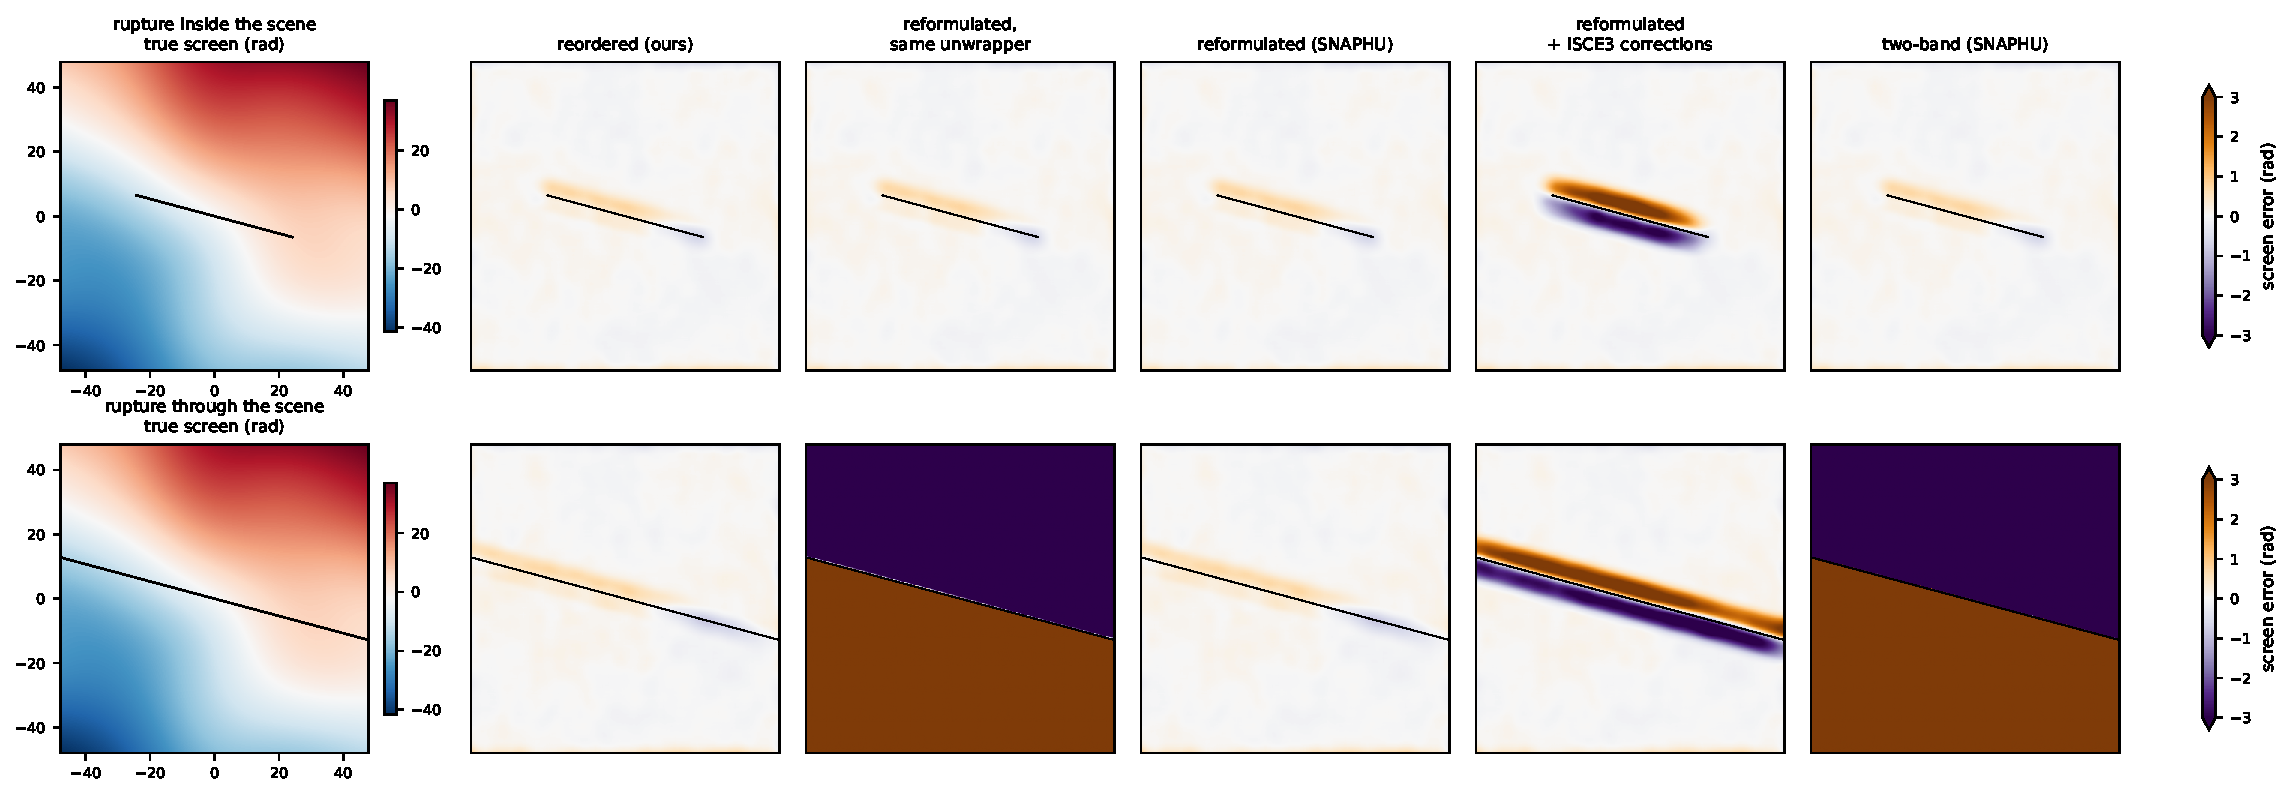
\includegraphics[width=\textwidth]{figures/fig_maps}
\caption{Screen errors (rad) on the two example scenes, 4\,m peak slip, one noise realization, for five of the eight
estimators. Top: a 50\,km rupture inside the scene. Bottom: a 160\,km rupture through it. Left: the true ionosphere.}
\label{fig:maps}
\end{figure}

\begin{figure}[t]
\centering
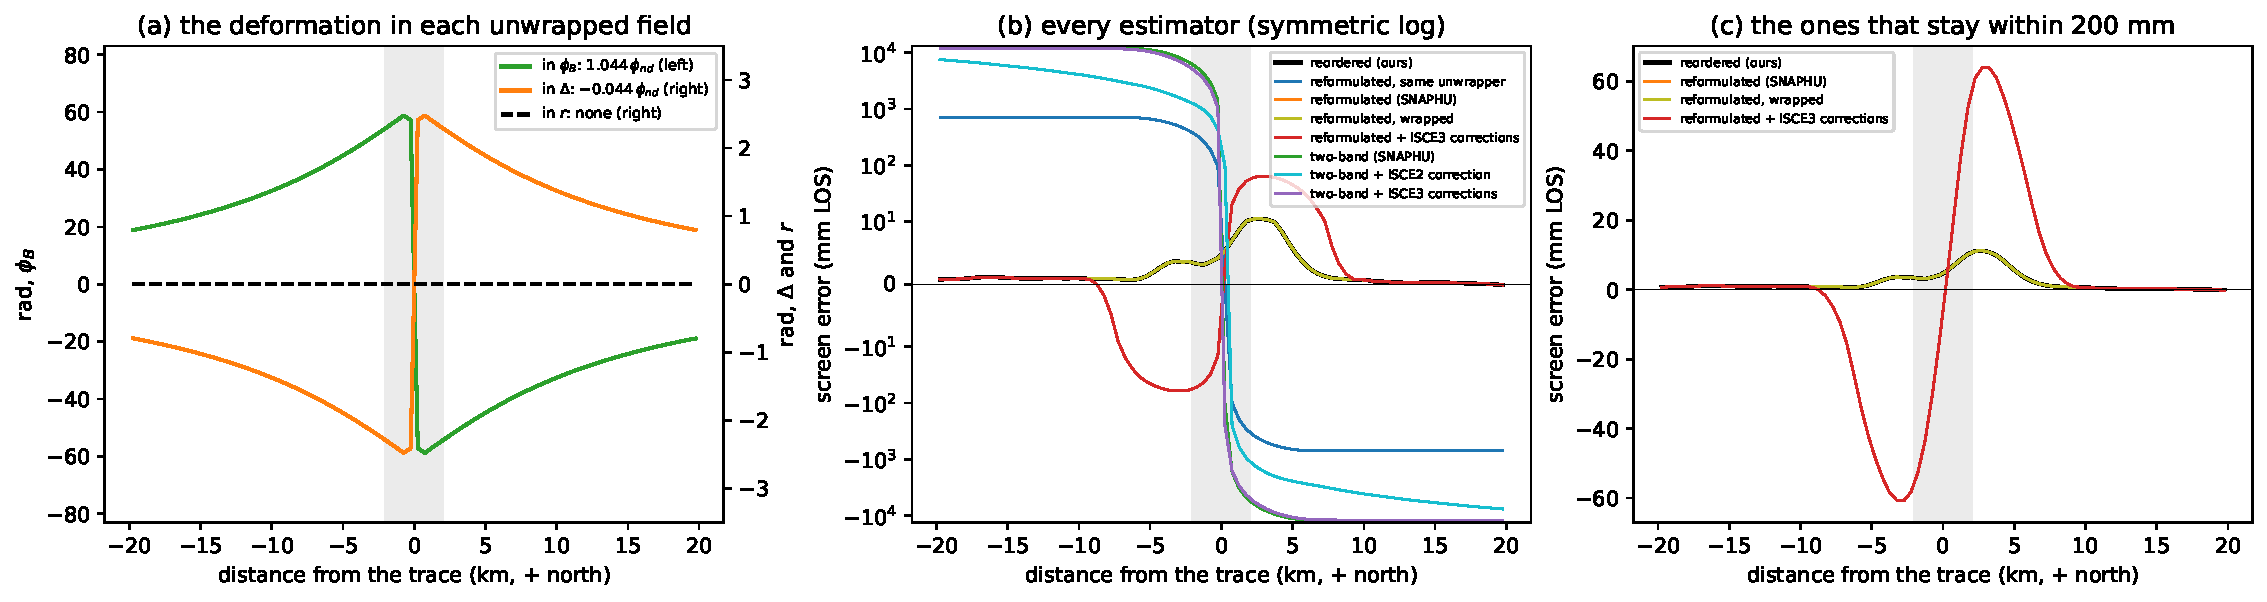
\includegraphics[width=\textwidth]{figures/fig_profiles}
\caption{(a) The deformation each form unwraps, across the through-going 4\,m rupture: all of it in $\phiB$, 4.4\%
in $\Delta$, none in $r$; grey is the excluded fault zone. (b, c) Each estimator's screen error across the trace, as
the median over 0.5\,km bins.}
\label{fig:profiles}
\end{figure}

\begin{figure}[t]
\centering
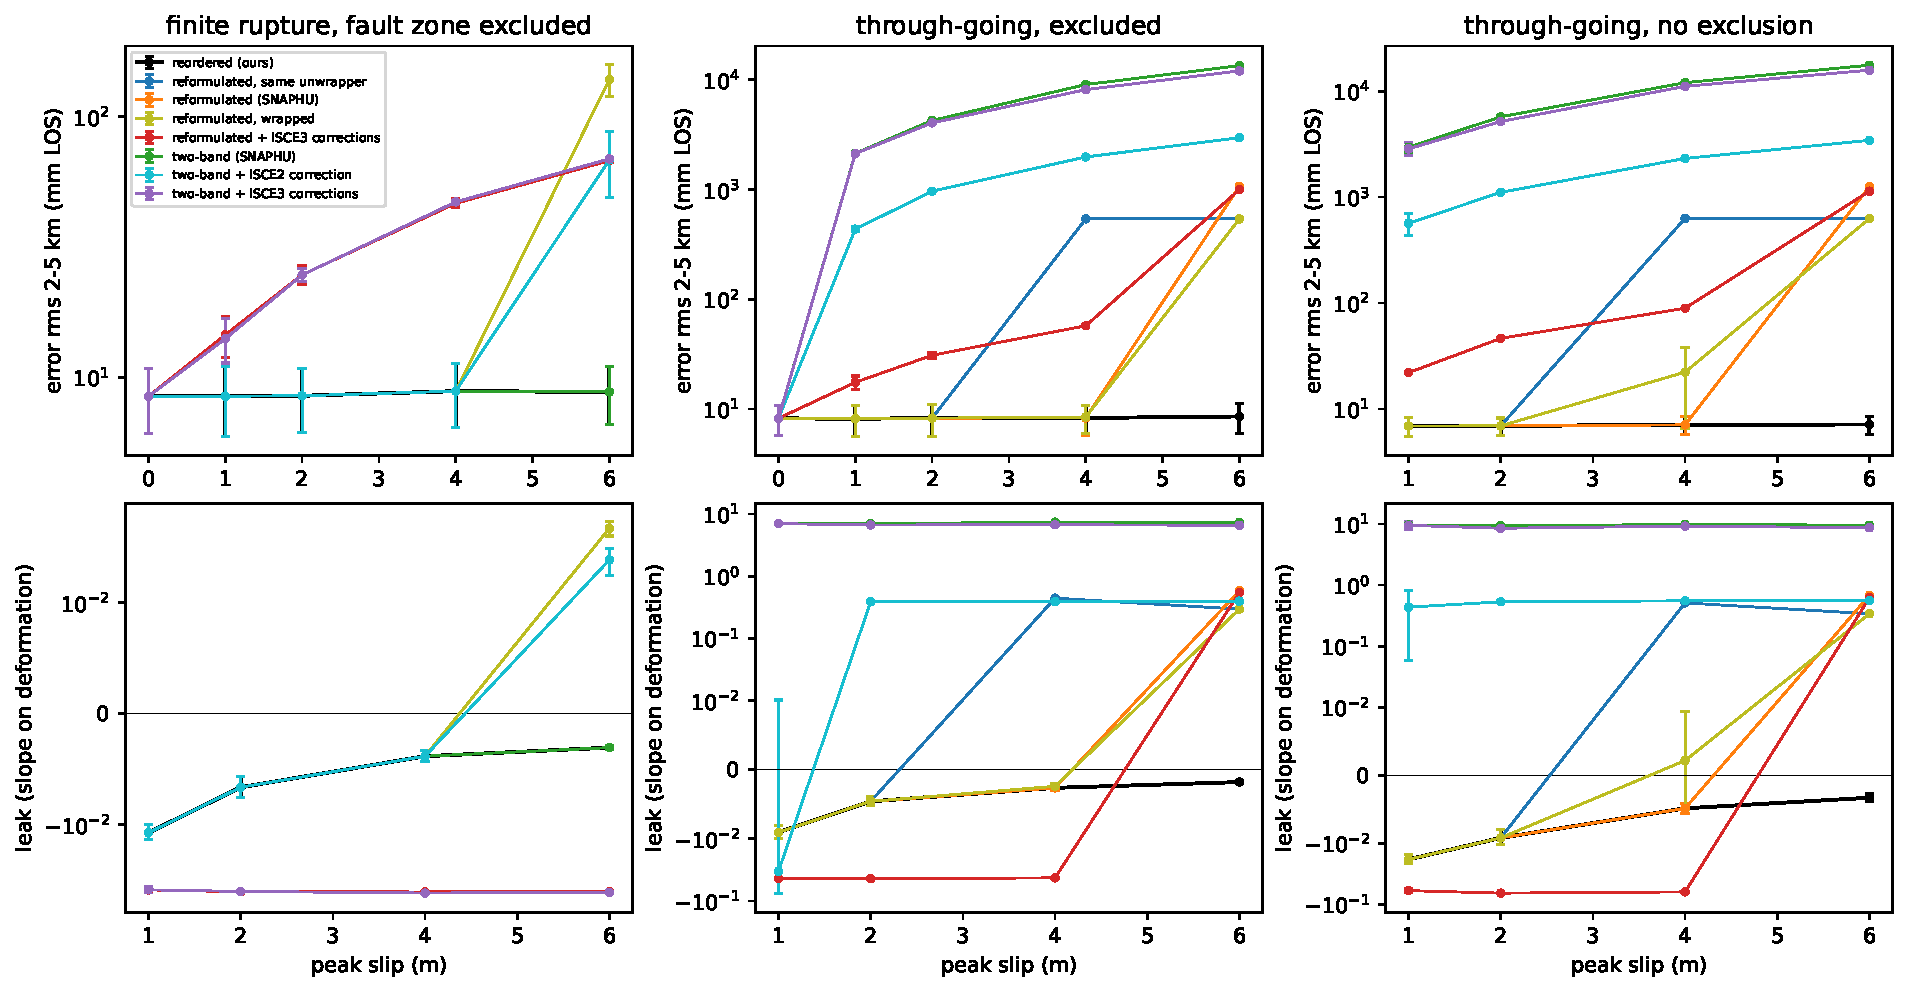
\includegraphics[width=\textwidth]{figures/fig_sweep}
\caption{Error 2--5\,km from the trace and leak against peak slip, mean and spread of three noise realizations. Left:
the rupture ends inside the scene. Middle: it runs through it. Right: as middle, without the fault-zone exclusion.}
\label{fig:sweep}
\end{figure}

\section{NISAR: the 2026 Venezuela and Panama earthquakes}
\label{sec:nisar}

\subsection{Data}
We use NISAR's L-band PR products in the 40\,+\,5\,MHz mode, HH polarization.
\begin{itemize}
  \item \textbf{Venezuela}, four 12-day pairs spanning the 24 June 2026 events on the San Sebasti\'an fault:
        ascending tracks 61 (18--30 June) and 162 (13--25 June), and descending tracks 54 (17--29 June) and 126
        (22 June -- 4 July). Two frames per track.
  \item \textbf{Panama}, descending track 141, 27 September -- 9 October 2026, frames 84 and 85, spanning the
        9 October $M_w$\,7.7 earthquake.
\end{itemize}
Each pair is the first date's PR GSLC and the second date's RSLC geocoded onto its grids
(Appendix~\ref{app:registration}). The main band is multilooked to 50\,m, filtered (adaptive Goldstein
\citep{goldstein1998radar}) and unwrapped with SNAPHU, with a cut along the mapped rupture where the rupture would
otherwise be crossed (Venezuela's airport segment, all of D141). D141's south block is tied to the north at 34
cycles, one more than our range offsets gave it, by the side band (Section~\ref{sec:sbtie}). Every estimator of Section~\ref{sec:synthetic} runs on the cells, main-band unwrapping, fault-zone exclusion
and filter that made our screens. The \texttt{ours} arm reproduces the saved production screens to $4\times10^{-6}$\,rad on every track. The PR GUNW
of the same pair, made by ISCE3's \texttt{main\_diff\_ms\_band} with \texttt{unwrap\_correction: True}, is binned onto
the same cells, with its frames levelled on their overlap.

There is no truth here. The leak is measured as in the earlier comparisons: the slope of the screen's 15\,km
high-pass on that of the non-dispersive phase ($\phiA$ minus our screen), within 10\,km of the trace. That uses our
own screen as the reference for what is deformation. A second statistic avoids this: each screen's difference from
ours near the fault and far from it, and its step across the trace.

\subsection{Results}
\paragraph{Panama D141.} The rupture runs into the Gulf of Montijo at its west end and out of the swath at its east,
so the main band was unwrapped with a cut along the trace, and the block south of it was tied at 34 cycles
(Section~\ref{sec:sbtie}). Across the
trace, the non-dispersive phase steps by 197\,rad between 2--4\,km north and south, 3.8\,m of LOS. The double
difference therefore has to step by $0.044\times197 = 8.7$\,rad, 1.38 cycles, across a gap that no data bridge.
Every reformulated arm puts the south block one cycle of $\Delta$ off: within 10\,km of the trace their screens differ
from ours by up to 72.9\,rad (69\,rad for the wrapped one), whichever unwrapper is used. That includes the GUNW recipe on our cells, with or
without the fault-zone exclusion (Table~\ref{tab:nisar}, Fig.~\ref{fig:d141}). The two-band arms are off by several
cycles of the side band. Their leaks are positive (+0.12 to +0.16 reformulated, +1.2 to +1.5 two-band) because the
block's offset correlates with the step. Ours leaks $+0.001$ and steps $-8$\,mm across the trace. On the offsets' tie
it leaked $-0.005$ and stepped 17\,mm: the filter's mixing of a wrong tie (Section~\ref{sec:sbtie}).

The GUNW product itself is not one of these arms. Its main band was unwrapped without a cut and is 32 cycles off
across the rupture, because SNAPHU went around its end. Its double difference was unwrapped on the GUNW's own grid,
across the decorrelated fault zone, and the correction passes then ran on both. What results is the copy described in
Section~\ref{sec:intro}: a leak of $-0.104$ ($r=-0.81$), a 433\,mm step across the trace, and a difference from ours of
294\,mm rms within 10\,km. Most of it is the main band's integers. Averaged onto our cells, the product's unwrapped
phase is 25 cycles below ours on the south block and 3--9 above it within 30\,km north of the trace (ours is tied by
the side band). With that main band, even the reordered estimate leaks $-0.061$ ($r=-0.70$), and the GUNW recipe
$-0.056$. The reordering does not protect a screen from a wrong main band, at 3.21\,rad per cycle; on D141 the
remedy is the cut and the tie.

\paragraph{Venezuela.} The four tracks see a rupture that runs along the coast. North of the trace is sea for much
of its length, and the airport's cut-off block is left out of the estimate, so no cross-fault integer has to be
recovered. There the forms agree, as on the benign synthetics.
\begin{itemize}
  \item The reformulated estimate with our unwrapper equals ours on every track. With SNAPHU it differs only in local
        patches (on A061, up to 31\,rad within 10\,km of the trace). Taken as wrapped, it fails on D126, where $\Delta$
        spans more than a cycle.
  \item The two-band forms fail on every track: the side band's own unwrapping is off by cycles over much of the scene.
  \item The correction passes leak on every track (Fig.~\ref{fig:nisar}b). The GUNW recipe on our cells moves
        main-band cycles at 0.03--0.24\% of the cells and leaks 0.009--0.019 more than ours with the exclusion, and
        0.018--0.048 more without it.
\end{itemize}
Ours is not at zero: $+0.009$ on A061, $-0.036$ on D126, $-0.003$ on A162 and $+0.037$ on D054. Every non-failing arm
shares that value on its track, so it is the metric's floor there, not leakage. On D126 the rupture runs along a
coastline, and the 15\,km high-pass of a field that ends at the coast correlates with that of the near-fault
deformation. D054 carries real ionospheric waves 15--30\,km apart, which its GUNW screen shows too.

The products leak more: $-0.083$ ($r=-0.72$) on A061, $-0.123$ ($-0.82$) on D126, $-0.045$ ($-0.62$) on A162 and
$-0.021$ ($-0.19$) on D054. Beyond ours, that is 0.042--0.092. Two tests narrow down where it comes from.
\begin{itemize}
  \item Unlike D141's, these products' main band agrees with ours: the two differ by a whole cycle at 0.14\% of the
        cells or fewer, and at 0.3\% or fewer within 10\,km of the trace. With the products' main band, our estimate
        is unchanged and the recipe's leak moves by at most 0.004.
  \item Widening our side-band cells in range to the products' footprint (the side band multilooked over 325\,m of
        slant range against the main band's 40\,m; a $[0.365, 1, 0.365]$ kernel matches the second moment) changes
        every arm's leak on these tracks by at most 0.004.
\end{itemize}
The recipe on our cells thus accounts for 25--52\% of the products' leak beyond ours, and neither the main band's
integers nor the footprint mismatch accounts for the rest. That rest lies in steps our matched cells do not
reproduce: the products' own grid, their double difference unwrapped and bridged there, and their frame-by-frame
processing. We leave its attribution open.

\begin{table}[t]
\centering
\caption{The estimators on NISAR data, on identical cells: leak (slope and correlation of the screen's 15\,km
high-pass on the non-dispersive phase's, within 10\,km of the trace), the screen's step from 2--4\,km south to
2--4\,km north, and its difference from ours (both less their median beyond 20\,km), within 10\,km and beyond
20\,km. All in mm of LOS.}
\label{tab:nisar}
\scriptsize
\setlength{\tabcolsep}{4pt}
\begin{tabular}{llrrrrr}
\toprule
scene & estimator & leak & $r$ & step & \multicolumn{2}{c}{difference from ours} \\
 & & & & (mm) & $<$10\,km & $>$20\,km (mm) \\
\midrule
D141 & reordered (ours) & 0.001 & 0.32 & -7.8 & 0.0 & 0.0 \\
 & reformulated, same unwrapper & 0.136 & 0.72 & -682.8 & 931.7 & 136.3 \\
 & reformulated (SNAPHU) & 0.163 & 0.77 & -834.6 & 925.4 & 136.5 \\
 & ISCE3 recipe, no exclusion & 0.131 & 0.74 & -672.7 & 904.9 & 136.4 \\
 & two-band (SNAPHU) & 1.540 & 0.81 & -7417.3 & 7421.1 & 1079.4 \\
 & PR GUNW & -0.104 & -0.81 & 433.0 & 294.1 & 38.6 \\
\midrule
A061 & reordered (ours) & 0.009 & 0.42 & 22.3 & 0.0 & 0.0 \\
 & reformulated, same unwrapper & 0.009 & 0.42 & 22.3 & 0.0 & 0.0 \\
 & reformulated (SNAPHU) & 0.013 & 0.02 & 13.0 & 73.0 & 0.2 \\
 & ISCE3 recipe, no exclusion & -0.039 & -0.59 & 24.9 & 9.4 & 0.1 \\
 & two-band (SNAPHU) & 0.844 & 0.53 & -3.0 & 278.7 & 11.8 \\
 & PR GUNW & -0.083 & -0.72 & 21.4 & 18.6 & 7.3 \\
\midrule
D126 & reordered (ours) & -0.036 & -0.47 & 108.8 & 0.0 & 0.0 \\
 & reformulated, same unwrapper & -0.036 & -0.47 & 108.8 & 0.0 & 0.0 \\
 & reformulated (SNAPHU) & -0.036 & -0.47 & 108.8 & 0.0 & 0.2 \\
 & ISCE3 recipe, no exclusion & -0.057 & -0.65 & 99.3 & 5.4 & 0.8 \\
 & two-band (SNAPHU) & 0.069 & 0.51 & 109.0 & 12.5 & 278.1 \\
 & PR GUNW & -0.123 & -0.82 & 64.2 & 18.8 & 10.2 \\
\midrule
A162 & reordered (ours) & -0.003 & -0.11 & 15.6 & 0.0 & 0.0 \\
 & reformulated, same unwrapper & -0.003 & -0.11 & 15.6 & 0.0 & 0.0 \\
 & reformulated (SNAPHU) & -0.003 & -0.09 & 15.5 & 0.2 & 0.3 \\
 & ISCE3 recipe, no exclusion & -0.025 & -0.45 & 17.6 & 5.0 & 0.4 \\
 & two-band (SNAPHU) & 1.515 & 0.55 & 10.8 & 310.8 & 560.5 \\
 & PR GUNW & -0.045 & -0.62 & 18.1 & 12.2 & 7.6 \\
\midrule
D054 & reordered (ours) & 0.037 & 0.39 & 1.4 & 0.0 & 0.0 \\
 & reformulated, same unwrapper & 0.037 & 0.39 & 1.4 & 0.0 & 0.0 \\
 & reformulated (SNAPHU) & 0.037 & 0.39 & 1.4 & 0.0 & 0.0 \\
 & ISCE3 recipe, no exclusion & 0.019 & 0.19 & -2.5 & 5.3 & 0.5 \\
 & two-band (SNAPHU) & 0.916 & 0.51 & -0.7 & 250.3 & 37.8 \\
 & PR GUNW & -0.021 & -0.19 & -16.8 & 11.1 & 8.2 \\
\bottomrule
\end{tabular}

\end{table}

\begin{figure}[t]
\centering
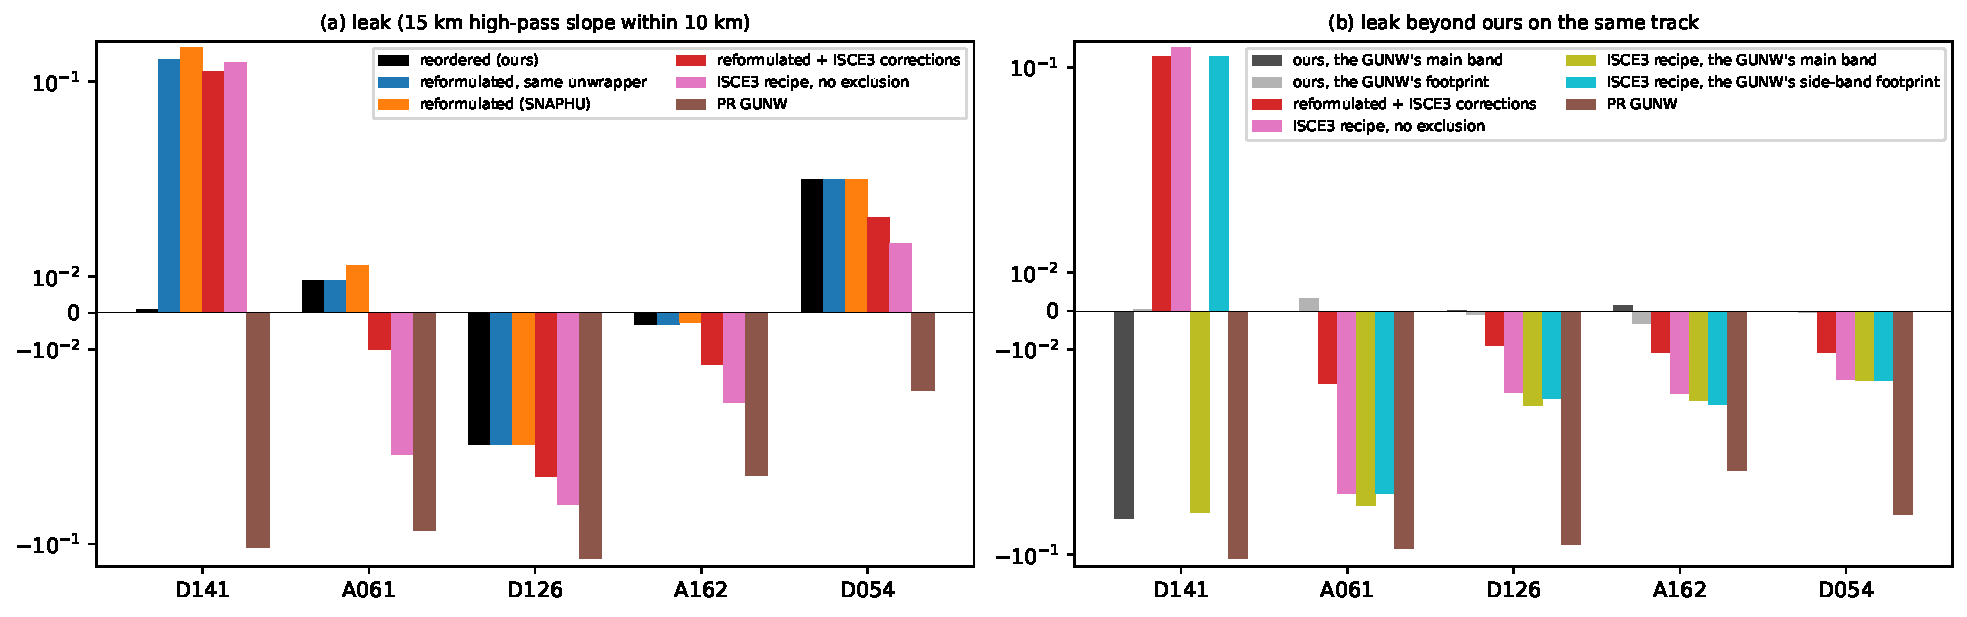
\includegraphics[width=\textwidth]{figures/fig_nisar}
\caption{The leak on the five NISAR tracks. (a) Each estimator on our cells, and the PR GUNW. (b) The leak beyond
ours on the same track, which removes each track's floor (the value every non-failing arm shares). It shows the GUNW
recipe on our cells, the same with the product's own main band or the product's side-band footprint, and the product.
Symmetric log scale.}
\label{fig:nisar}
\end{figure}

\begin{figure}[t]
\centering
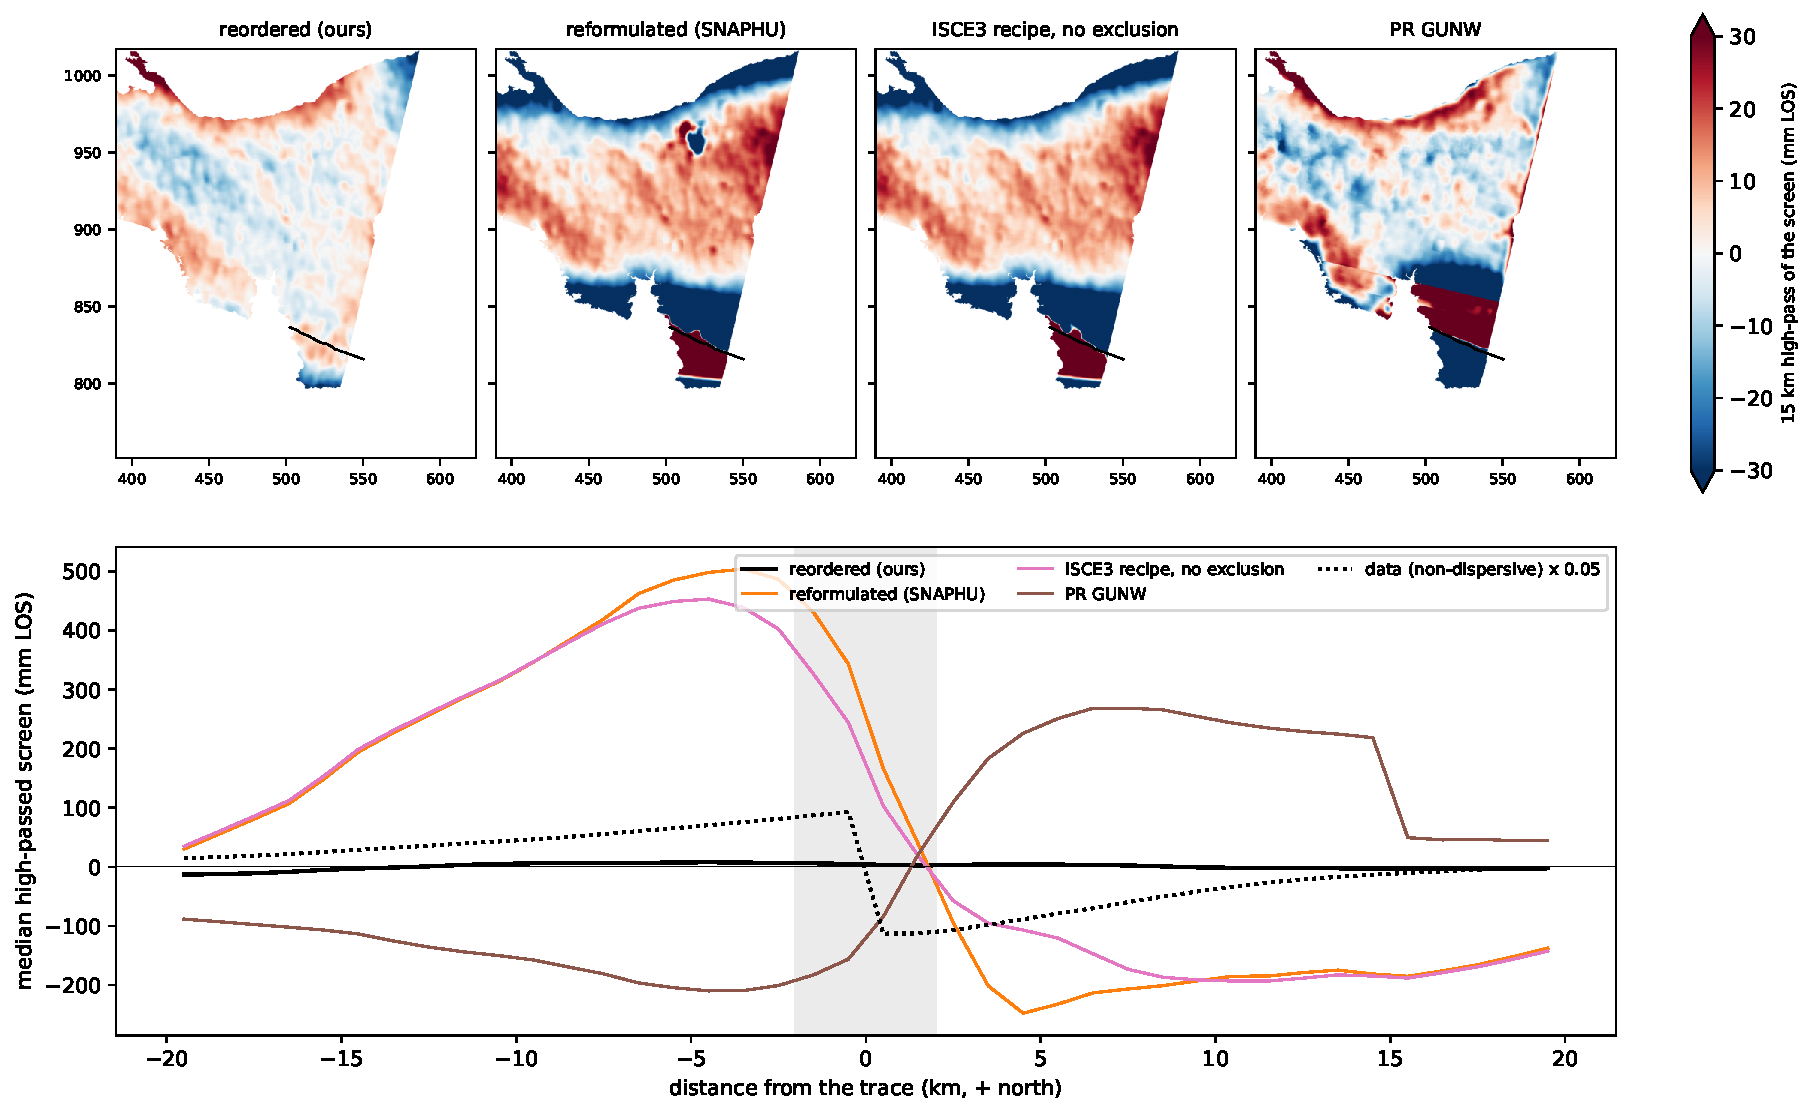
\includegraphics[width=\textwidth]{figures/fig_d141}
\caption{Panama D141. The 15\,km high-pass of four screens on identical cells: ours, the reformulated estimate with
SNAPHU, the GUNW recipe on our cells (no exclusion), and the PR GUNW product. Below: their median across the
trace, with the data's high-pass ($\times0.05$) for reference.}
\label{fig:d141}
\end{figure}

\section{The side band ties a cut-off block}
\label{sec:sbtie}

Where a rupture splits the scene, the main band is unwrapped with a cut along the trace, and the block the cut
isolates carries an arbitrary integer. The Panama pipelines tie it with the range offsets. They read
$m = (4\pi/\lambda)\,\rho_\mathrm{off} - \phiA$, which holds the block's cycles and twice the ionosphere but no
deformation, fit a plane to $m$ 6--12\,km from the trace on each side, and compare the two planes at the trace. The
fractional parts of those ties are large: $-0.35$ (D141 on the cut of Section~\ref{sec:nisar}), $-0.13$ (D141 on the
production cut), $+0.33$ (D040), $+0.41$ (A076) and $-0.43$ (A004). This section shows that the side band ties the
block itself, and that on three of the four Panama pairs it finds those ties one cycle short. The offsets themselves
agree with it when they are read the same way. What puts the ties a cycle short is comparing two far-field planes at the
trace.

\subsection{Principle}
A block whose main-band integer is off by $\epsilon$ carries $2\pi c_0\,\epsilon = 3.21\,\epsilon$\,rad of extra raw
estimate (Table~\ref{tab:integers}): the scaled main band is taken out of the wrapped side band, so all of each wrong
cycle but $c_0$ of it wraps away. Nothing else in the raw estimate steps across the gap between two blocks. The
ionosphere is continuous across a fault zone or a strait a few kilometres wide, and the deformation is not in the
estimate. The raw estimate's step across the gap therefore measures $\epsilon$. We tile the boundary into windows of
20\,km and fit, in each,
\begin{equation}
  \hat d = P(x, y) + \delta\,\mathbf{1}_B + n, \qquad e = -\frac{\delta}{2\pi c_0},
  \label{eq:tie}
\end{equation}
over the cells of both blocks within 12\,km of the other. $P$ is a quadratic shared by both sides, so the ionosphere's
gradient and curvature are fitted across the gap rather than extrapolated from one side. The weights are each cell's
Cram\'er--Rao variance, reweighted by Tukey's biweight so that patches with local main-band cycle errors, each
3.21\,rad off, do not move the step. $e$ is the number of cycles to add to block $B$, and the tie is the median of $e$
over the windows (\texttt{split\_spectrum.\allowbreak block\_cycles}). A second estimator replaces $P$ by a Gaussian
process (Mat\'ern 3/2 plus a plane, its length and noise scales by restricted maximum likelihood in each window, the
cells as medians over $3\times3$) and checks the first.

The two ties are equally exposed to the ionosphere. A misfit of $\Delta$\,rad in the ionosphere modelled across the
gap reads as $\Delta/3.21$ cycles in the side band, and as $2\Delta/2\pi = \Delta/3.14$ cycles in $m$, which carries
the ionosphere twice and the integer at $2\pi$. They differ in everything else. The raw estimate is precise to
0.5--1\,rad per 240\,m cell and comes from the cells that make the screen. The registration offsets the pipelines tie
with are noisier, about 0.2\,m of slant range per correlation window, or 10\,rad of $m$. They are also smoothed on each
side of the trace and filled where the correlation was culled; that turns out not to matter
(Section~\ref{sec:panamaties}).

Using the bands' separation to join separately unwrapped regions is not new. \citet{libert2017split} do it at X band,
where the ionosphere is negligible, by reading each region's absolute phase from its split-band phase. At L band the
ionosphere dominates that absolute phase \citep{gomba2016toward}. What we use instead is the ionosphere's continuity
across the gap.

\subsection{Validation}
\paragraph{Synthetic ruptures.} The through-going synthetic of Section~\ref{sec:synthetic}, with the oracle main
band, so the answer is 0; three seeds, 0 and 4\,m of slip, and five variants (the default ionosphere, far-field
coherence 0.35, patchy decorrelation, travelling waves of 3\,rad at 25\,km, and a rough ionosphere of 8\,rad at 8\,km).
Putting the south block's main band one cycle off moves every one of its cells' raw estimates by exactly 3.2092\,rad,
through the whole chain, so planted ties are exact shifts: they come back to $3\times10^{-5}$ cycles.
\begin{itemize}
  \item Without local cycle errors, the polynomial reads within 0.21 of the truth (rms 0.08--0.12) in every variant but
        the rough one, and kriging within 0.11 (rms 0.03--0.06) in every one. Slip makes no difference.
  \item The rough ionosphere is where the polynomial fails. Over 20 ionospheres of each kind, with white noise in place
        of the rest of the chain, its rms is 0.09 (default), 0.11 (waves) and 0.44 (rough), where 5 of the 20 ties are
        a cycle off; kriging's is 0.02, 0.03 and 0.05, and none is off by more than 0.08.
  \item With local cycle errors in 15\% of one side's cells 2--6\,km from the gap, in 1\,km patches, the polynomial
        stays within 0.15 of the truth (0.32 in the rough ionosphere). In 35\% they bias both estimators by $+0.2$ to $+0.4$ on
        average, and a few ties come out a cycle off: the robust fit cannot reject a third of the cells that matter most.
  \item Leaving out the cells within 6\,km of the gap does not help: the extrapolation across 12\,km is worse
        (rms 0.27--0.44), with or without local errors.
\end{itemize}

\paragraph{Fake boundaries on real data.} Straight lines through one block of each of eight scenes (the four Panama
north blocks and the four Venezuela main regions), at least 15\,km from the trace, at four orientations every 12\,km,
each with the 2\,km on either side left out as a fault zone is. Nothing steps there, so every estimate should be 0.
Over 6082 windows, $|e|$ has a median of 0.035 and a 95th percentile of 0.26 (0.15 without D054), with no bias (mean
$+0.001$); 1.7\% of windows exceed 0.5. The tail has two causes, both visible in maps of the raw estimate. Most windows
that exceed 0.5 on A004, A061, A162 and D126 hold sharp-edged patches where the main band itself is off by one to
three cycles, on coastal strips, islands and a river floodplain: there the side band is right, and the fake boundary
is not a null. On D054, an evening pass, the ionosphere carries waves of 10--20\,km wavelength and several radians,
and a window whose line runs along a wave front reads up to two cycles; 4.7\% of its windows exceed 0.5. Taken as a tie is, the median over a
line's windows, no line reads a wrong integer: of 565 lines with two or more windows, the largest $|e|$ is 0.47, and
the 17.7\% of D054's lines whose windows disagree by more than 0.25, or whose median is more than 0.25 from an
integer, are flagged as ambiguous.

\paragraph{A rupture with the main band unwrapped through it.} On Venezuela's A162 and D054 the main band joins the
two sides around the rupture's west end, and the north side has data along the first 60\,km of it, so the right answer
is 0. The side band reads $+0.02$ on A162 (windows $+0.02$, $-0.04$, $+0.14$) and $-0.04$ on D054 ($+0.75$, $-0.23$,
$-0.04$), and kriging $0.00$ and $+0.03$. D054's first window sits in its ionospheric waves.

\paragraph{Two unwrappings.} D141's main band was also unwrapped without a cut, with a phase model built from the
range offsets taken out before unwrapping and put back after. That puts 92.5\% of the south block exactly two cycles
below the cut and tied unwrapping. The side band reads $+3.0$ to $+3.2$ in every window of the uncut one and $+0.6$ to
$+1.7$ in those of the tied one, whose near-fault cells carry local cycle errors the uncut one does not; their medians
differ by 1.8 (20\,km windows) to 2.1 (16\,km). Through the exact two cycles between them, the uncut unwrapping also
says the tied one needs $+1.06$.

\paragraph{Not the deformation.} Across the Panama ruptures the main band steps by $-70$ to $-208$\,rad (2--4\,km
either side) on the descending tracks and by $+125$ to $+199$\,rad on the ascending A076, while $e$ is $+1$ on all
three. A step that leaked the deformation would change sign with the look direction. The south block's offset is also
the same at every distance from the trace (Fig.~\ref{fig:tie}a), where a leak would decay with the deformation.

\subsection{The Panama ties}
\label{sec:panamaties}
Table~\ref{tab:tie} lists the south blocks of the four Panama pairs as the production screens cut them (D141, D040 and
A076 on the 20 October trace, A004 on the 13 October one). On D141, D040 and A076 the side band reads $+1.19$, $+1.28$
and $+0.93$, and kriging $+1.12$, $+1.00$ and $+0.91$. Each of the pipelines' ties is one cycle short, and the blocks'
integers are 27, 21 and $-22$. D040's polynomial median is 0.28 from an integer, because one of its three windows, at the east
end beside the trace's eastern branches, reads $+2.15$; it is flagged ambiguous, and kriging and the cells 6--12\,km from the gap
($+1.21$) agree on one cycle. A004's south block lies against the swath's near-range edge, where band A's partially
focused strip is left out, and only one window has data on both sides ($-0.30$, kriging $-0.11$): it is consistent with
the pipelines' tie but does not confirm it. On the cut of Section~\ref{sec:nisar}, D141's tie is 34, not 33.

\paragraph{The offsets agree, read the same way.} In the pipelines' geometry (a plane per side, 6--12\,km from the
trace, the two compared at it) the side band and $m$ differ by 0.6--1.5 cycles. Their combination $m + 2\hat\phi_{io}$,
which cancels both the ionosphere and the block's integer, steps by as much across the three ruptures. It looks as if
the offsets and the phase disagreed there by 7--18\,cm of range.

But read with the side band's own estimator, the same offsets agree with it (Table~\ref{tab:tie_readings}). That
estimator fits one quadratic over both blocks and a step on the south one, using cells from 2\,km of the trace. It reads
the correlator's offsets at $+0.84$, $+1.06$ and $+0.99$ cycles (the smoothed ones at $+0.84$, $+1.71$ and $+0.84$),
against the side band's $+1.19$, $+1.28$ and $+0.93$. It is the planes that differ. Each is fitted to one side alone and
extrapolated across at least 12\,km of gap. Read that way the same offsets give $+0.12$, $+0.67$ and $+0.28$ (smoothed:
$-0.08$, $+0.85$ and $+0.33$), while the side band stays at $+1.31$, $+1.44$ and $+1.00$.

A far-field plane does not carry $m$ to the trace. Within 2\,km of the trace, $m$ departs from its own far-field plane
by up to 1.0--1.5 cycles (A076, D040, A004). Used as a phase model for D141's uncut unwrapping, the offsets put the south
block two cycles from where their planes put it.

Three further checks rule out the alternatives.
\begin{itemize}
  \item \emph{The pipelines' smoothing.} The correlator's offsets before it (the ROFF lattices geocoded, with only gross
        outliers removed) match the smoothed ones to 0.3\,cm in the median (robust sd 9\,cm). They also read the same:
        $+0.84$, $+1.06$ and $+0.99$ from 2\,km.
  \item \emph{The cells.} On D141's per-pixel cells (Section~\ref{sec:pixel}), with the south block at 34, the side band
        reads $+0.37$ ($+0.11$ from 6\,km). On the cells as summed it reads $+0.19$ ($+0.10$). A bias of the summed
        cells would read $-1$.
  \item \emph{A third, independent set of offsets.} The GUNWs' own pixel offsets cannot be one here: they are not
        measurements. Their run configurations switch on ISCE3's polynomial rubbersheet, which fits one quadratic per
        frame to a $200\times200$ grid of the dense offsets, for the along-track and the slant-range offsets each, and
        resamples the secondary with it. The offset layers the products carry are that quadratic; a cubic in map
        coordinates fits them to within 3\,mm rms. They hold no coseismic step, so a tie read from them is the step left
        uncancelled, and beyond 20\,km, on coherent ground, they follow only the long-wavelength part of ours (to about
        8\,cm). The Antarctic products (Section~\ref{sec:antarctica}) take ISCE3's other branch and keep the dense
        field.
\end{itemize}
The offsets remain the weaker reading. From 6\,km they give $+0.40$, $+1.00$ and $+0.64$, and their windows scatter
several times more than the side band's (D040's run from $+0.24$ to $+4.55$). They agree with the side band, but they do
not settle the tie on their own.

\paragraph{The side band is not biased by the step.} The side band steps nowhere else: not at 565 fake boundaries, nor
across the Venezuela rupture whose integer is known. Those controls are weaker than the Panama case, though: their main
band steps by at most 26\,rad 2--4\,km from the trace, against 70--208\,rad here. A bias of the side band that grows with
the step and keeps its sign for both look directions would escape them. The Antarctic pairs of
Section~\ref{sec:antarctica} supply that control, in one look direction. Across a glacier's shear margin the
non-dispersive phase steps by 74--188\,rad. There the side band and the range offsets, read the same way, tie the cut-off
component alike, window by window: 8.95 against 8.90 cycles, and 7.97 against 7.96.

A wrong tie does not reach the slip inversion through the block's level, which a per-block offset absorbs (59\,mm per
cycle after the screen). It does through the filter, which fills the excluded zone from both blocks and mixes them
(Fig.~\ref{fig:tie}d). Correcting the three ties by a cycle raises the corrected LOS (positive toward the satellite)
just north of the trace by 36--38\,mm, by 27--29\,mm at 2--3\,km and by 8--11\,mm at 6--8\,km, and lowers it just
south by 18--20\,mm, by 10--13\,mm at 2--3\,km. The production screens carry that 5--6\,cm fake step, opposite in
sign, where the inversion reads the shallow slip.

\begin{table}[t]
\centering
\caption{The cut-off blocks' ties: cycles to add to the main band of each south block, by the side band (median over
20\,km windows of the robust polynomial, and of kriging) and by $m$ read with the same estimator (cells 2--12 and
6--12\,km from the gap), beside the range-offset tie the pipelines applied (their planes; Table~\ref{tab:tie_readings}
reads the offsets three ways). A162 and D054 are controls: their main
band runs through the rupture, and the answer is 0.}
\label{tab:tie}
\setlength{\tabcolsep}{4pt}
\begin{tabular}{lrrrrrrr}
\toprule
 & \multicolumn{2}{c}{range offsets} & \multicolumn{3}{c}{side band, $e$} & \multicolumn{2}{c}{$m$, as the side band} \\
\cmidrule(lr){2-3}\cmidrule(lr){4-6}\cmidrule(lr){7-8}
pair & tie & measured & polynomial & kriging & windows & 2--12\,km & 6--12\,km \\
\midrule
D141 & 26 & 25.87 & 1.19 & 1.12 & 2 & 0.84 & 0.19 \\
D040 & 20 & 20.33 & 1.28 & 1.00 & 3 & 1.71 & 1.03 \\
A076 & -23 & -22.59 & 0.93 & 0.91 & 4 & 0.84 & 0.57 \\
A004 & -21 & -21.43 & -0.30 & -0.11 & 1 & 0.05 & -0.16 \\
D141, Section 5's cut & 33 & 32.65 & 1.32 & -- & 2 & -- & -- \\
A162 (no cut) & -- & -- & 0.02 & 0.00 & 3 & -- & -- \\
D054 (no cut) & -- & -- & -0.04 & 0.03 & 3 & -- & -- \\
\bottomrule
\end{tabular}

\end{table}

\begin{table}[t]
\centering
\caption{The Panama ties read three ways from three fields, in cycles to add to the pipelines' offset ties (26, 20 and
$-23$). The fields are the raw dispersive estimate (the side band) and $m$, from the registration offsets as the
pipelines smoothed them and from the correlator's offsets before smoothing (gross outliers removed). Each is read with
the side band's estimator using cells from 2\,km and from 6\,km of the trace, and as the pipelines read it: a plane per
side, 6--12\,km from the trace, compared at it.}
\label{tab:tie_readings}
\small
\setlength{\tabcolsep}{3.5pt}
\begin{tabular}{lrrrrrrrrr}
\toprule
 & \multicolumn{3}{c}{side band} & \multicolumn{3}{c}{offsets, smoothed} & \multicolumn{3}{c}{offsets, raw} \\
\cmidrule(lr){2-4}\cmidrule(lr){5-7}\cmidrule(lr){8-10}
pair & 2\,km & 6\,km & planes & 2\,km & 6\,km & planes & 2\,km & 6\,km & planes \\
\midrule
D141 & 1.19 & 1.05 & 1.31 & 0.84 & 0.19 & -0.08 & 0.84 & 0.40 & 0.12 \\
D040 & 1.28 & 1.21 & 1.44 & 1.71 & 1.03 & 0.85 & 1.06 & 1.00 & 0.67 \\
A076 & 0.93 & 0.95 & 1.00 & 0.84 & 0.57 & 0.33 & 0.99 & 0.64 & 0.28 \\
\bottomrule
\end{tabular}

\end{table}

\begin{figure}[t]
\centering
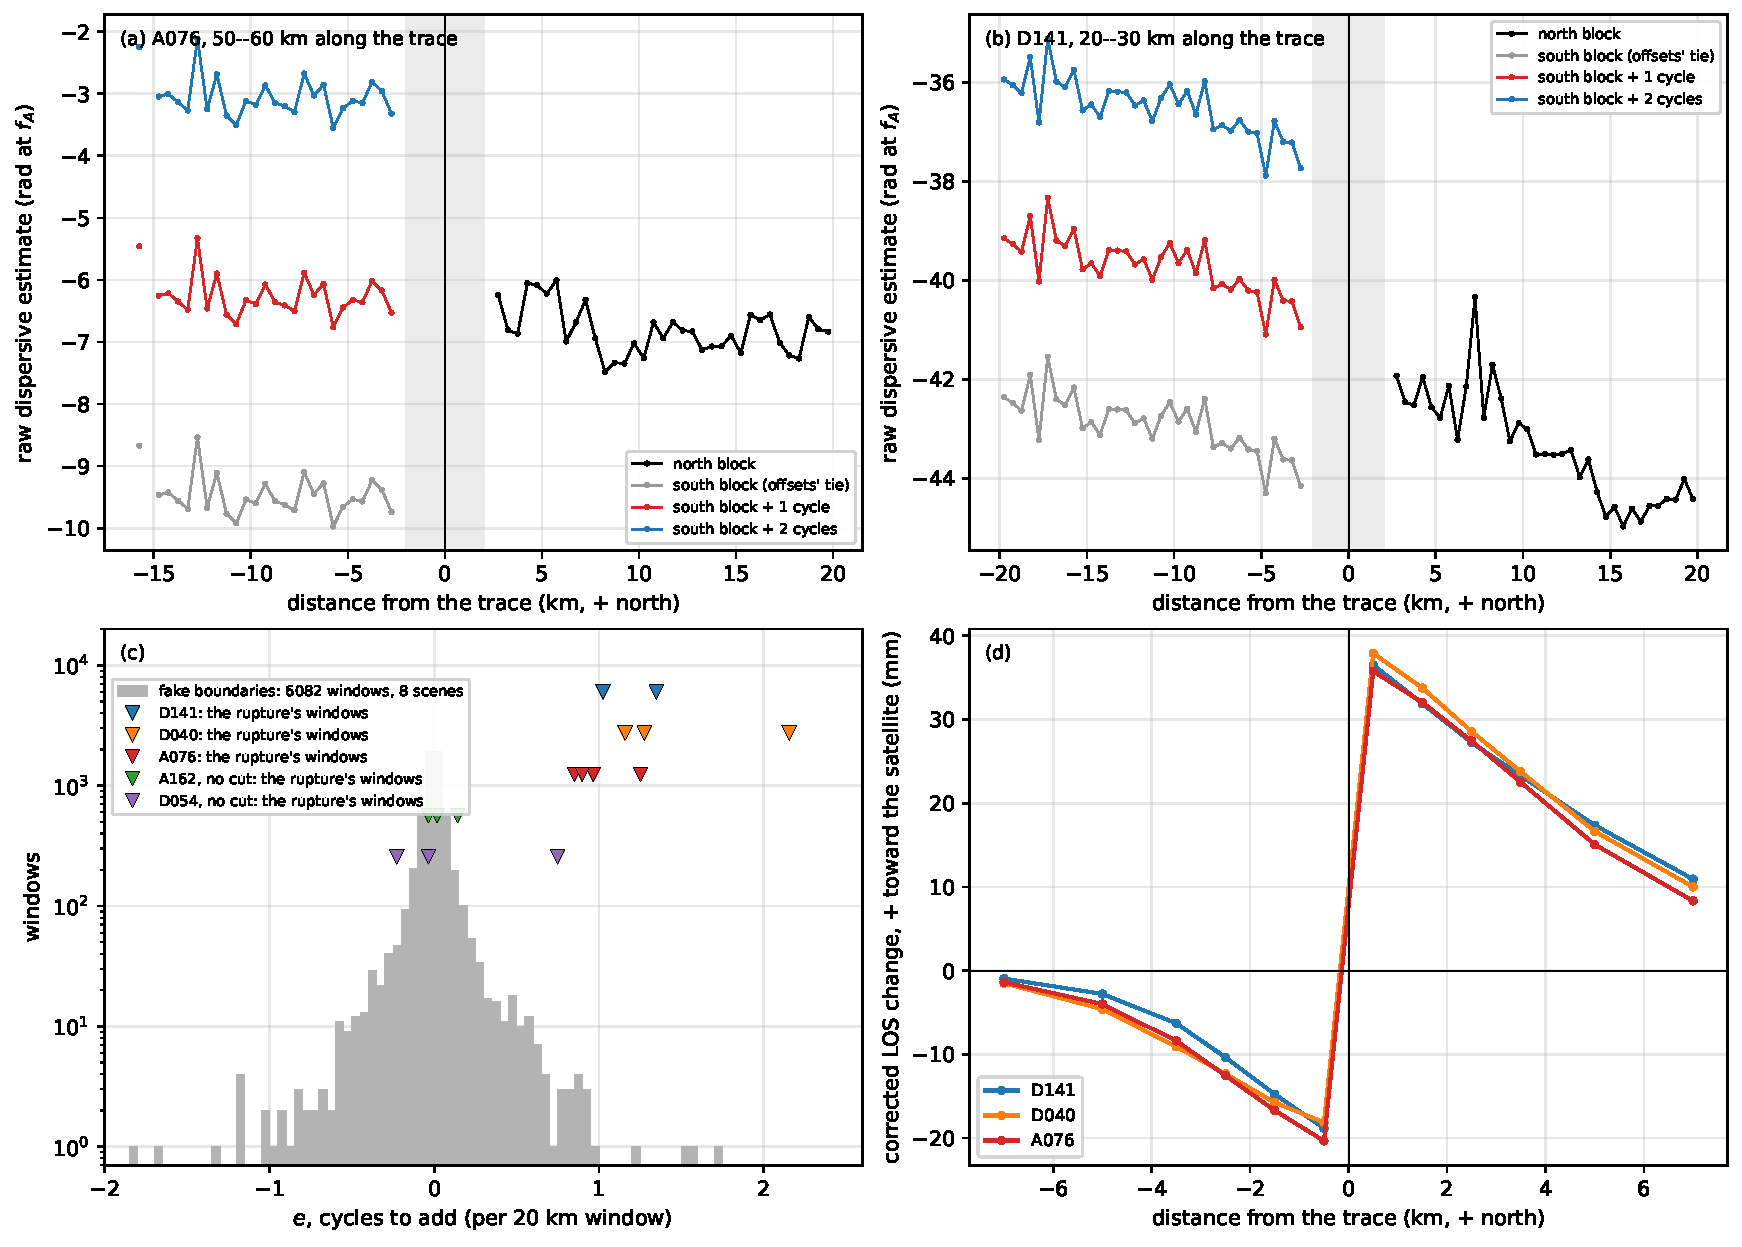
\includegraphics[width=\textwidth]{figures/fig_tie}
\caption{The side-band tie. (a, b) The raw dispersive estimate across the trace, median in 0.5\,km bins over 10\,km of
the trace, with the south block on the pipelines' offset tie and one and two cycles up. (c) $e$ on fake boundaries in eight
scenes (grey), and the windows along the real ruptures: one cycle on D141, D040 and A076, zero on the Venezuela
controls. (d) What adding one cycle to each south block does to the corrected LOS, beyond each block's constant: the
fake step the production screens carry, with the opposite sign.}
\label{fig:tie}
\end{figure}

\section{Near the trace: the fill, the filter, the cells and the integers}
\label{sec:nearfield}

On the synthetics, the reordered estimate's error near a rupture does not depend on the slip
(Section~\ref{sec:synthetic}). It is about 16\,mm of LOS inside the excluded fault zone and 7--9\,mm at 2--5\,km, the
same with no slip at all. Three parts of the estimator make it, and each can be changed: the fill's width, the filter's
weighted mean, and, where the deformation is steep, the cells themselves. Changed together, they bring that error
down to the far field's (Table~\ref{tab:nearfield}). Real data then say how much of it matters. On real ionosphere the
fills differ by about a millimetre, and next to the D141 rupture the screen is set by the main band's local integers
instead. The production screens of Sections~\ref{sec:nisar} and \ref{sec:sbtie} use none of the changes below.

\subsection{A fill matched to the gap}
\label{sec:fill}
Masked cells are filled by a local plane before the final Gaussian (Section~\ref{sec:estimator}). The production fill
uses one width, $\sigma = 10$\,km, chosen to reach across NISAR's partially focused near-range strip, where the screen
has to be extrapolated $\sim$11\,km from one side. Across a fault zone the data lie on both sides, and a narrower plane
should then follow a curved ionosphere better.

On synthetic ionospheres it does (Table~\ref{tab:fill}). The ionospheres are the default one, a rough one of 8\,rad at
8\,km and travelling waves of 3\,rad at 25\,km, with 0.7\,rad of noise per cell. In a 2\,km fault zone a 1.5\,km plane
misses by 2.0, 11 and 6\,mm rms, the 10\,km plane by 15, 60 and 29\,mm. The narrowest planes are best in every gap with
data around it, up to a 15\,km bay. Only deep in a one-sided strip do wider planes help, and there no plane does well:
30--130\,mm at 8--12\,km in. The plane's weighted data centroid tells the two cases apart: it stays near a cell inside
a gap with data on both sides, and moves away by about the distance to the data in a one-sided one. Each filled cell
therefore takes the narrowest of a ladder of planes whose data centroid lies within $1.5\sigma$ of it, blending into
the next width by $3\sigma$.

Real ionosphere is smoother at 2--10\,km than these synthetics, and its cells are noisier. We cut fake gaps out of
the raw estimates of the eight production screens of Section~\ref{sec:sbtie}: 34 windows of 100\,km, at least 15\,km
from a trace. Each window held a 40\,km fault zone of half-width 1, 2 or 4\,km at a random orientation, or had
everything beyond a line removed. We then refilled each gap and compared the result with the same filter run on all the
window's data (Table~\ref{tab:fill}, Fig.~\ref{fig:nearfield}b, c).
\begin{itemize}
  \item In 1--2\,km zones every fill errs by 1.1--3.1\,mm. A 2.6\,km plane, or a ladder that starts at it (2.6, 5 and
        10\,km), is best; the production plane is 0.6--1.1\,mm worse.
  \item The ladder that starts at 1.5\,km is too narrow for real data: 3.5--7\,mm in a 4\,km zone, against 2.1--3.6\,mm
        for the 2.6\,km ladder and 2.8--4.7\,mm for the production plane.
  \item At a one-sided edge, 6--10\,km planes are best (2.5--5\,mm at 0--8\,km), with the 2.6\,km ladder close behind
        (3.2--7.4\,mm). The narrowest plane and ISCE3's zero-order guide are 3--7 times worse there.
\end{itemize}
A matched fill is therefore worth about a millimetre in a real fault zone. Section~\ref{sec:integers} shows what it can
cost.

\subsection{A filter that does not lag where its weights change}
\label{sec:order}
ISCE3's final step is a Gaussian mean of the raw estimate, weighted by each cell's inverse Cram\'er--Rao variance. A
fault's damage zone lowers the coherence toward the trace, so the weights fall toward it. The mean's centroid then
moves away from the trace on both sides, and the screen lags the ionosphere's gradient in opposite directions on the two
sides. On the synthetic scene with D141-like near-field deformation, the raw estimate is unbiased to $\pm$2\,mm on each
side of the trace, while the filtered screen is 7--15\,mm high north of it and 8--11\,mm low south of it at 0.5--5\,km
(Fig.~\ref{fig:nearfield}a). With uniform weights, or with a weighted local plane through the same truncated kernel,
the asymmetry is gone.

The plane is a weighted Savitzky--Golay step: at each cell, the least-squares plane through the cells within the
kernel, weighted by the kernel times their inverse variances, evaluated at the cell. It is exact for a linear field,
whatever the weights, and equals the weighted mean wherever the weights are symmetric about the cell. Its variance
$e_0^\top M^{-1} N M^{-1} e_0$, with $M$ the weighted moments and $N$ the same moments under the squared kernel, takes
the place of the mean's in ISCE3's output sigma. \citet{piromthong2026ionospheric} fit such planes, with Gaussian
distance weights, against the same lag at scene edges. Next to a rupture it arises inside the data. With the matched
fill and the plane, the synthetic error within 2\,km of the trace falls to 2.0\,mm and at 2--5\,km to 1.5\,mm. The step
across the trace falls from 6.9 to 0.6\,mm, at 4\,m of slip as at none, against 1.3\,mm beyond 20\,km
(Table~\ref{tab:nearfield}).

How much the lag matters depends on the ionosphere's gradient where the weights change. Away from ruptures, on the real
fake gaps, the plane changes the error by at most 0.4\,mm. Next to the D141 rupture it moves the screen by at most
3\,mm, with the main band as cut or repaired (Section~\ref{sec:integers}).

\subsection{The main band out of every pixel}
\label{sec:pixel}
The cells sum each band's pixels before the scaled main band is taken out of the side band's cell phase. Where the
deformation changes by several radians across a 240\,m cell, the sums decorrelate. Their phases are then means of the
fringes that the two bands weight differently: the bands' speckle is independent, and the side band's pixels are eight
times wider in range. That difference enters $r$, and $d = r/k$ amplifies it 11.6 times. On a noise-free pair whose
fringes change by 2--20\,rad/km, the per-cell raw estimate errs by 0.25--2.5\,rad rms (5--48\,mm) per cell. North of
D141's trace the main band changes by a median 14--24\,rad/km within 2\,km. There only 2.5--18\% of the cells within
5\,km keep a coherence above 0.2 in both bands, against 19--64\% south of the trace.

Instead, \texttt{gslc\_cells} can take the caller's unwrapped main band $M$, interpolated to each pixel, out of every
pixel of both bands, scaled to each band's frequency, before the sums:
\begin{equation}
  \rho_A = \arg \sum_j a_j\, e^{i(\psi_{A,j} - M_j)}, \qquad
  \rho_B = \arg \sum_j b_j\, e^{i(\psi_{B,j} - (\fB/\fA) M_j)}, \qquad
  r = \W\!\left(\rho_B - \frac{\fB}{\fA}\,\rho_A\right),
  \label{eq:pixel}
\end{equation}
where $a_j$ and $b_j$ are the pixels' amplitudes. Pixel by pixel, $\psi_{B,j} - (\fB/\fA)\psi_{A,j} = k\,d_j$ exactly,
so the deformation leaves the sums before they are formed. What remains of the model's own error inside a cell enters
only as the difference of its two band-weighted means. On the noise-free pair, the raw estimate's error falls to
0.002\,rad, the precision of the model's interpolation. The model's integers are still the caller's, at 3.21\,rad per
cycle. Its sub-cycle errors no longer matter: with the true phase as the model, or with the main band's own pixels
after a one-pixel Gaussian, the synthetic screens agree to 0.05\,mm. The Gaussian multilook and the Goldstein filter
that precede the main band's unwrapping therefore reach the screen only through its integers. In both forms of the
cells, the values are the GSLCs' own pixels.

With the Okada field alone, which changes by $\sim$3\,rad/km at the trace, the two forms of the cells give the same
screen. With the D141-like near field, the per-pixel cells keep 34, 58, 96 and 100\% of the cells at 0--0.5, 0.5--1,
1--2 and 2--5\,km from the trace, against 6, 19, 45 and 83\% per cell. Their raw error at 2--5\,km is 17\,mm, against
29\,mm per cell and 15\,mm far from the trace. On D141 itself they double the cells kept north of the trace within
5\,km: 20 against 5\% at 0.5--1\,km, 35 against 18\% at 2--5\,km (Fig.~\ref{fig:nearfield}d). Those are the cells whose
main band is least certain.

\subsection{The main band's local integers}
\label{sec:integers}
On D141 the fill moves the screen near the trace by more than it moves the synthetics. A 2.6\,km plane and both
ladders raise it there by 7--16\,mm against the production screen, on both sides of the trace
(Fig.~\ref{fig:nearfield}e). The per-pixel cells add up to 4\,mm north of it, and the first-order filter moves it by
at most 3\,mm. The raw estimate shows why. Within 6\,km north of the trace it sits $\sim$15\,mm
above its own continuation from farther out, and it steps across the trace by 20--30\,mm. That step matches the 0.32
cycles left after the side band's whole-cycle tie (Section~\ref{sec:sbtie}).

The same pair was also unwrapped without the cut (v5 of Section~\ref{sec:sbtie}). Cell by cell, the two unwrappings'
integers differ beyond each block's modal difference north of the trace on 78\% of the cells within 1\,km, 62\% at
1--2\,km, 42\% at 2--4\,km and 18\% at 4--6\,km, and on 3\% or fewer beyond 6\,km. South of the trace they differ on
8--15\% beyond 1\,km and 33\% within it. Each such cell carries 3.21\,rad of raw estimate per cycle. When those cells
take the uncut unwrapping's integers, every recipe comes within 5\,mm of the production screen
(Fig.~\ref{fig:nearfield}f). The production screen itself moves by 2.4\,mm or less: its 10\,km fill averages the
near-trace cells away. The narrow fills and the extra cells follow them.

Neither unwrapping is known to be right near the trace. What the comparison shows is the order of things. Near a real
rupture the screen is set by the main band's local integers, at 3.21\,rad (62\,mm) per cycle and cell. The fill, the
filter and the cells refine it by a few millimetres once those integers are right. Until they are, the production
recipe's wide fill and fault-zone exclusion are the robust choice. The side band could check the integers patch by
patch near the trace, as it checks a cut-off block's in Section~\ref{sec:sbtie}. We leave that for later.

\begin{table}[t]
\centering
\caption{The near-trace recipe, one change at a time, on the through-going synthetic rupture at 4\,m of slip (mean
of five noise realizations): error rms in mm of LOS within 0--2, 2--5 and 5--10\,km of the trace, and the error's
2--4\,km step across it. Left: the Okada field alone. Right: with rough near-field deformation as large as D141's
(median 16--21\,rad/km within 1\,km of the trace). The error beyond 20\,km is 1.3\,mm with the first-order filter
and 2.1\,mm without it. The main band is the truth's.}
\label{tab:nearfield}
\setlength{\tabcolsep}{4pt}
\begin{tabular}{lrrrrrrrr}
\toprule
 & \multicolumn{4}{c}{Okada field only} & \multicolumn{4}{c}{with D141-like near field} \\
\cmidrule(lr){2-5}\cmidrule(lr){6-9}
recipe & 0--2 & 2--5 & 5--10\,km & step & 0--2 & 2--5 & 5--10\,km & step \\
\midrule
production (v6) & 15.6 & 7.5 & 1.8 & 6.9 & 19.0 & 10.5 & 4.3 & 11.9 \\
+ fill matched to the gap & 4.4 & 3.5 & 1.7 & 5.5 & 4.6 & 5.9 & 4.1 & 9.7 \\
+ first-order filter & 2.0 & 1.5 & 1.3 & 0.6 & 2.6 & 2.0 & 1.3 & 0.8 \\
+ main band out per pixel & 2.0 & 1.5 & 1.3 & 0.7 & 2.2 & 1.7 & 1.3 & 0.3 \\
+ no fault-zone exclusion & 1.5 & 1.2 & 1.3 & 0.5 & 1.6 & 1.3 & 1.3 & 0.2 \\
\bottomrule
\end{tabular}

\end{table}

\begin{table}[t]
\centering
\caption{The fills, rms error in mm of LOS. Synthetic ionospheres (eight of each, 0.7\,rad of noise per cell): inside
a 2\,km fault zone, and 4--8\,km into a one-sided 12\,km strip. Real ionosphere (34 windows of 100\,km in eight NISAR
screens, against the same filter on all the data): inside fake fault zones of half-width 1, 2 and 4\,km, and in a
one-sided strip.}
\label{tab:fill}
\small
\setlength{\tabcolsep}{3.5pt}
\begin{tabular}{lrrrrrrrrr}
\toprule
 & \multicolumn{4}{c}{synthetic ionospheres} & \multicolumn{5}{c}{real ionosphere, fake gaps} \\
\cmidrule(lr){2-5}\cmidrule(lr){6-10}
 & \multicolumn{3}{c}{2\,km zone} & edge & \multicolumn{3}{c}{zone half-width} & \multicolumn{2}{c}{edge} \\
\cmidrule(lr){2-4}\cmidrule(lr){5-5}\cmidrule(lr){6-8}\cmidrule(lr){9-10}
fill & default & rough & waves & 4--8\,km & 1\,km & 2\,km & 4\,km & 0--4\,km & 4--8\,km \\
\midrule
plane, 1.5 km & 2.0 & 10.8 & 6.1 & 37.2 & 1.1 & 1.8 & 5.4 & 18.6 & 34.0 \\
plane, 2.6 km & 2.9 & 17.0 & 9.2 & 20.9 & 1.1 & 1.8 & 2.8 & 6.0 & 33.1 \\
plane, 4 km & 4.5 & 25.8 & 13.9 & 12.2 & 1.3 & 1.9 & 2.9 & 3.9 & 9.6 \\
plane, 10 km (production) & 14.8 & 59.8 & 28.6 & 29.2 & 1.7 & 2.7 & 3.7 & 3.3 & 5.1 \\
ladder 1.5--3--6--12 km & 2.0 & 10.8 & 6.1 & 15.5 & 1.1 & 1.8 & 4.4 & 6.4 & 7.8 \\
ladder 2.6--5--10 km & 2.9 & 17.0 & 9.2 & 15.5 & 1.1 & 1.8 & 2.8 & 4.6 & 7.4 \\
ISCE3's guide & -- & -- & -- & -- & 1.3 & 2.0 & 5.1 & 10.5 & 23.3 \\
\bottomrule
\end{tabular}

\end{table}

\begin{figure}[t]
\centering
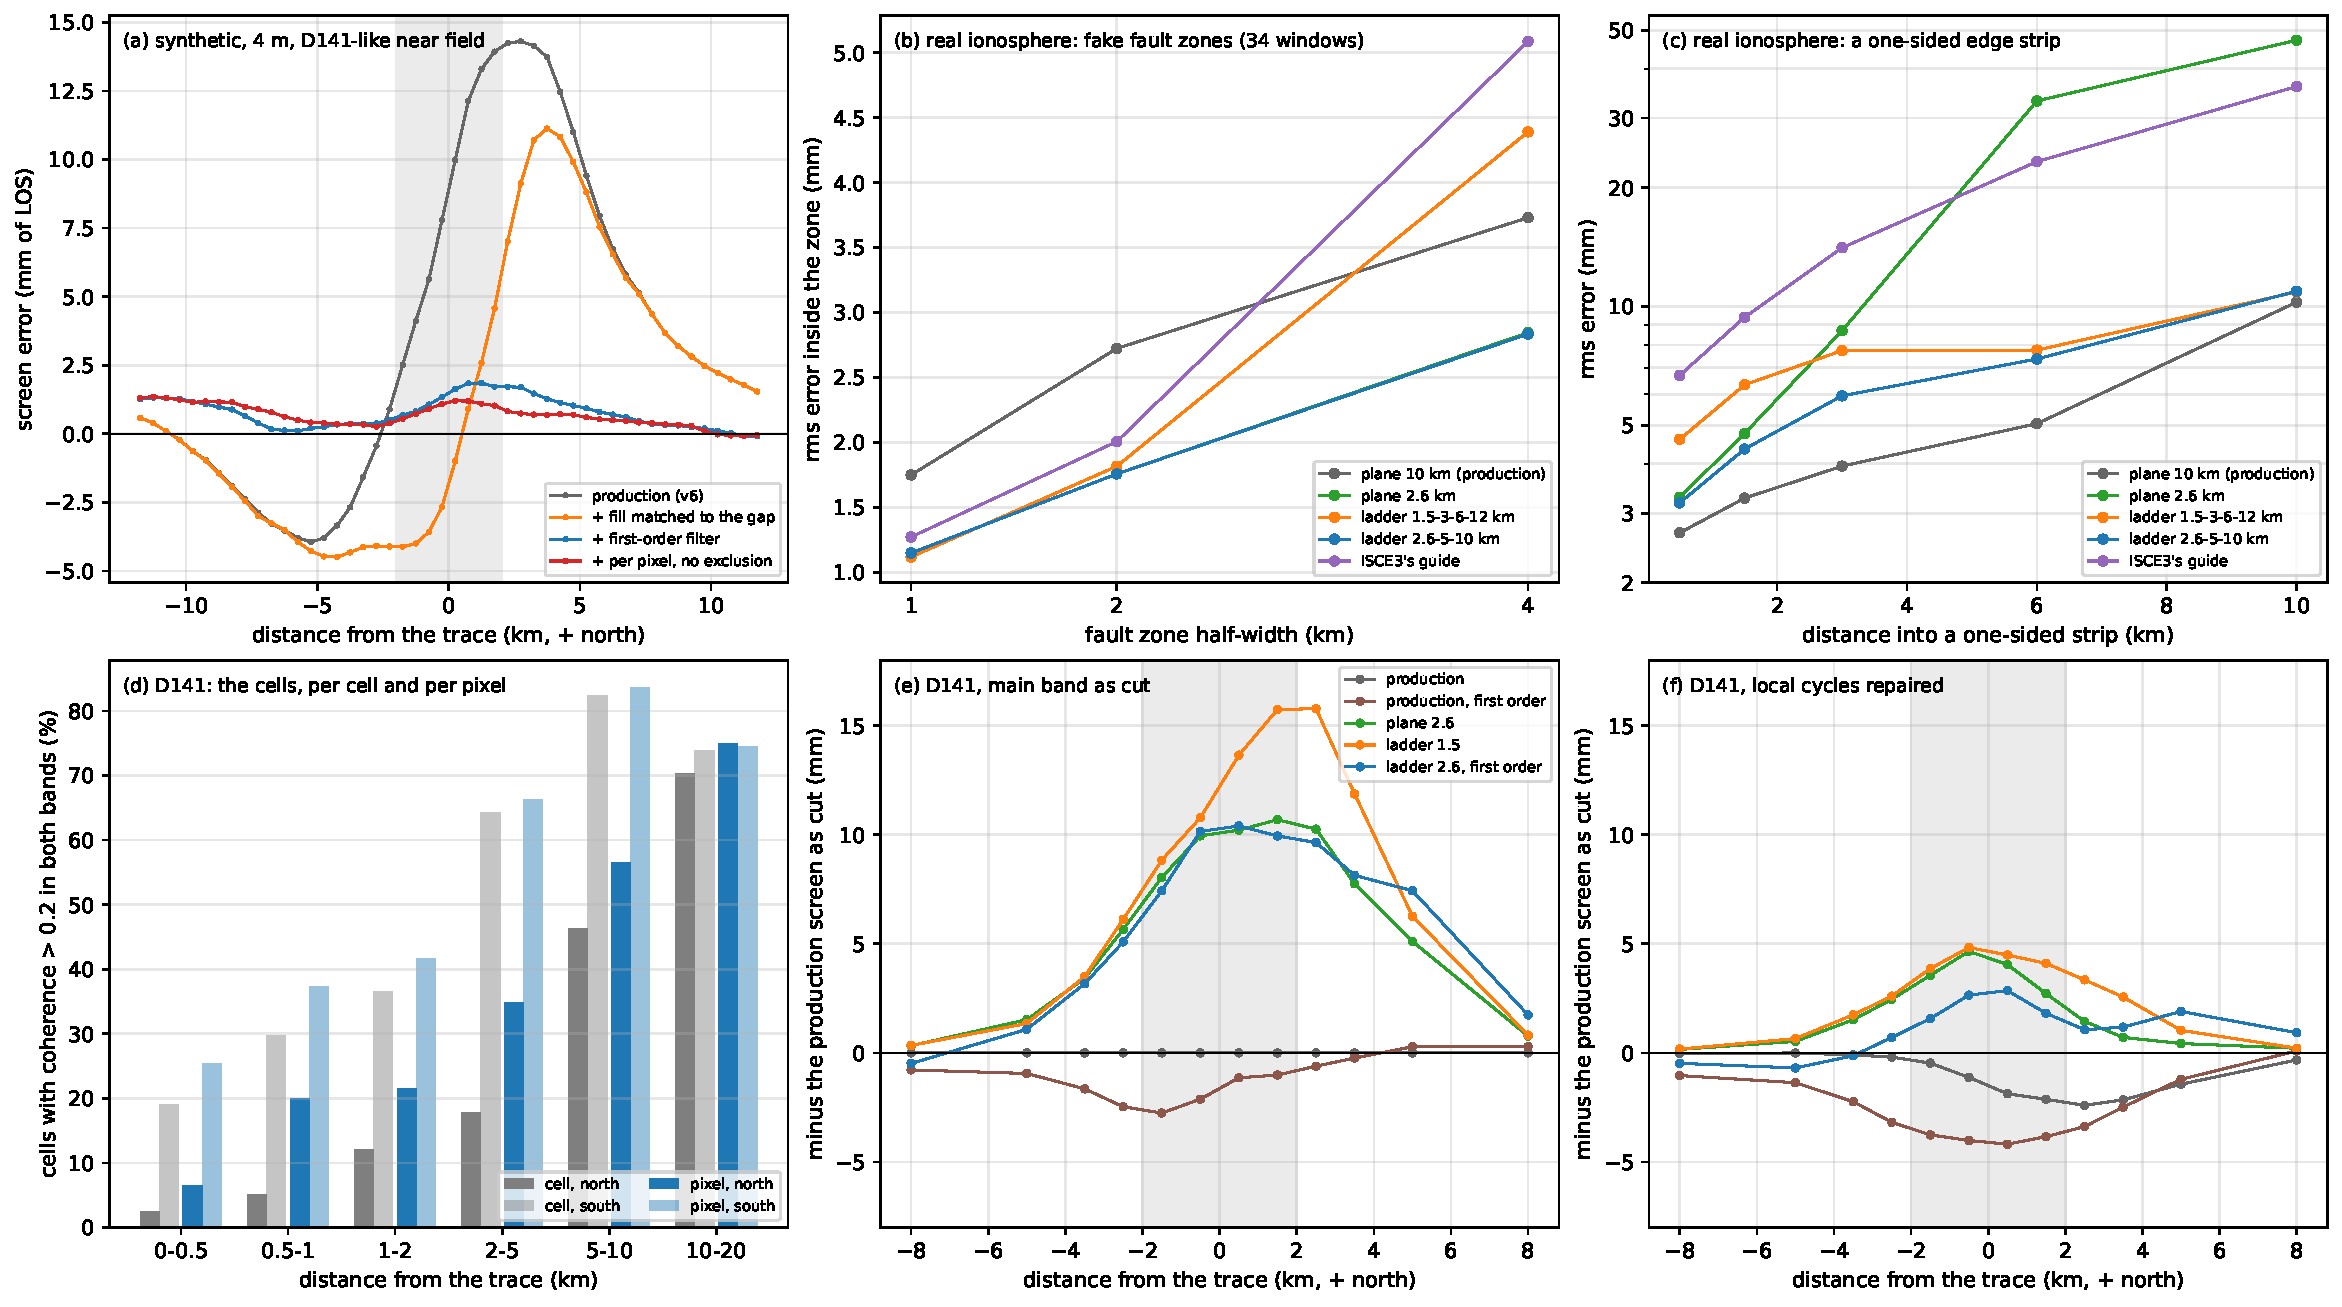
\includegraphics[width=\textwidth]{figures/fig_nearfield}
\caption{Near the trace. (a) The synthetic screen's error across the trace, D141-like near field, 4\,m of slip, one
change at a time; grey is the excluded zone. (b, c) The fills on real ionosphere: fake fault zones of 1--4\,km
half-width, and a one-sided strip. (d) D141: the cells with coherence above 0.2 in both bands, summed per cell and with
the main band taken out per pixel. (e, f) D141: each recipe's screen minus the production screen, with the main band
as cut and with its local cycles taken from the uncut unwrapping.}
\label{fig:nearfield}
\end{figure}

\section{Ice: the Antarctic pairs of nisarErrors}
\label{sec:antarctica}

\citet{joughin2026nisarerrors} compared the ionosphere corrections of NISAR's PR products with those of GrIMP, the
processing that turns NISAR interferograms into ice-velocity maps \citep{joughin2018grimp}, on two pairs over Greenland
and two over Antarctica. Over Greenland their main finding is a carrier error. ISCE3 registers the second date to the
ionosphere's azimuth shift, and the Doppler carrier turns that shift into a phase that scales with frequency. No
split-spectrum form removes it, and it is not considered here. Over Antarctica, on track 94 descending, frame 129
(80.2--82.9$^\circ$S, 13--33$^\circ$W, grounded ice upstream of the Filchner Ice Shelf), they found two things.
\begin{itemize}
  \item The RUNW's screen is about 40\,rad off over part of the second of its two connected components, between the
        component boundary and a glacier's shear margin.
  \item The unwrapped phase is split between the components. GrIMP fixes the split from its velocity map, at $-7$
        cycles in both pairs.
\end{itemize}
Against GrIMP's own velocity synthetic, the RUNW's corrected phase leaves a residual of 21.5 and 21.9\,rad (robust 26.8
and 26.6), and GrIMP's leaves 2.61 and 2.59 (2.20 and 2.00).
\authnote{\citet{joughin2026nisarerrors} is a public draft in a code repository; check with its author before citing
it.}

For an interferogram, a glacier's shear margin is what a strike-slip rupture is: a steep step in the non-dispersive
phase, decorrelated over kilometres, that the unwrapper may not cross. The products were made with the recipe of
Section~\ref{sec:nisar} (ISCE3 0.25.16, \texttt{main\_diff\_ms\_band}, \texttt{unwrap\_correction: True}, read from
their run configuration). These pairs therefore test Section~\ref{sec:theory}'s account on data that hold no
earthquake, and the range offsets give an independent check.

\subsection{Data and processing}
The pairs are 19--31 August and 31 August -- 12 September 2026, in NISAR's 40\,+\,5\,MHz mode, HH. They go through the
pipeline of Section~\ref{sec:nisar} with three differences.
\begin{itemize}
  \item The registration field is the GUNW's own pixel offsets, the field ISCE3 applied, plus the first date's TEC and
        solid-earth-tide shift (Appendix~\ref{app:registration}). Gross outliers, more than 5\,m from their 600\,m
        neighbourhood, are removed first.
  \item The main band is the product's own unwrapped phase, so that the comparison isolates the screen. Fast ice puts
        several fringes into a 240\,m cell, so the cells take it out of every pixel before the sums
        (Section~\ref{sec:pixel}). Its sign was checked on the 20\,km box where it changes fastest: the cells' median
        coherence there is 0.55 with it taken out, 0.49 without it, and 0.31 with its sign flipped (pair 1).
  \item There is no fault zone to exclude.
\end{itemize}
Our screen is made three ways: with the main band's integers as delivered, from the main component alone, and with the
other component re-tied to it by the side band (Section~\ref{sec:sbtie}). The product's screen is binned onto the same
cells. The estimators of Section~\ref{sec:synthetic} also run on these cells, with the absolute cell phases rebuilt from
the model's cell mean. Their \texttt{ours} reproduces the tied screen to 0.002\,rad rms.

\begin{table}[p]
\centering
\caption{The Antarctic pairs (track 94 descending, frame 129).
\emph{The product's screen minus ours}, cell by cell: component 1's offset in main-band cycles (3.21\,rad), the block's
in cycles of the double difference (72.96\,rad), and what is left.
\emph{The split of component 1}, read three ways in the same 17 windows along the boundary, beside GrIMP's fix, and the
non-dispersive step across the gap there.
\emph{Over the tributary's trunk}: the plateau left after the integers, what ISCE3's correction passes add there on our
cells, and the leak (slope, and $r$ in brackets, of the screen's 15\,km high-pass on the non-dispersive phase's) with
the cells within 5\,km of either integer step left out.
\emph{The offsets' ionosphere} minus each screen: where the screens differ, $(\phiA - k\rho_\mathrm{off})$ smoothed over
3\,km and calibrated on ours; over the frame, $(\phiA - k\rho_\mathrm{off})/2$ uncalibrated, both smoothed over 6\,km, a
median and a plane removed per screen.
\emph{nisarErrors' residual metric} against an ITS\_LIVE synthetic, on slow grounded ice ($<$50\,m/yr).
\emph{Pair 1 minus pair 2}: the corrected phases' difference, a median and a plane removed, on the pixels coherent in
both.}
\label{tab:antarctica}
\small
\setlength{\tabcolsep}{4pt}
\begin{tabular}{lrr}
\toprule
 & pair 1 & pair 2 \\
 & 19--31 Aug & 31 Aug--12 Sep \\
\midrule
\multicolumn{3}{l}{\emph{The product's screen minus ours}} \\
component 1, in main-band cycles & 9.013 & 8.004 \\
the block, in double-difference cycles & 1.0006 & 0.9995 \\
\quad its area (km$^2$) & 11\,980 & 11\,304 \\
left after the integers: robust sd (rad) & 0.13 & 0.13 \\
\quad area beyond 3\,rad (km$^2$) & 5\,400 & 5\,078 \\
\addlinespace
\multicolumn{3}{l}{\emph{The split of component 1, in main-band cycles}} \\
side band (median of 17 windows) & 8.95 & 7.97 \\
range offsets, $\phi_A - k\rho_\mathrm{off}$: the GUNW's & 8.90 & 7.96 \\
\quad ours, a gross-outlier cull only & 9.06 & 8.15 \\
ITS\_LIVE, slow ice within 20\,km & 8.01 & -- \\
GrIMP's fix \citep{joughin2026nisarerrors} & 7 & 7 \\
non-dispersive step across the gap (rad) & 74--188 & 80--188 \\
\addlinespace
\multicolumn{3}{l}{\emph{Over the tributary's trunk, 5--20\,km outside the block}} \\
product $-$ ours $-$ integers (rad) & 6.50 & 5.44 \\
\quad in main-band cycles & 2.03 & 1.70 \\
ISCE3's passes on our cells (rad) & 3.60 & 3.52 \\
leak away from the integer steps: product & -0.066 (-0.65) & -0.066 (-0.67) \\
\quad ours & 0.002 (0.09) & 0.001 (0.03) \\
\addlinespace
\multicolumn{3}{l}{\emph{The offsets' ionosphere minus each screen (rad)}} \\
product above ours by $>$3\,rad: minus ours / minus product & -0.28 / -5.60 & -0.32 / -4.91 \\
product below ours by $>$3\,rad: minus ours / minus product & +0.34 / +3.47 & +0.27 / +3.01 \\
over the frame, rms (6\,km): product / repaired / ours & 18.85 / 1.29 / 0.63 & 18.85 / 1.21 / 0.68 \\
\addlinespace
\multicolumn{3}{l}{\emph{Phase minus an ITS\_LIVE synthetic, slow ice: $\sigma$ / robust $\sigma$ (rad)}} \\
uncorrected & 3.50 / 3.15 & 2.09 / 1.69 \\
the product's screen & 15.19 / 14.24 & 15.05 / 14.08 \\
the product's, integers repaired & 4.04 / 1.36 & 3.97 / 1.44 \\
ours & 1.84 / 1.22 & 1.84 / 1.21 \\
\addlinespace
\multicolumn{3}{l}{\emph{Pair 1 minus pair 2, a median and plane out: $\sigma$ / robust $\sigma$ (rad)}} \\
uncorrected & \multicolumn{2}{c}{3.94 / 4.13} \\
the product's screen & \multicolumn{2}{c}{1.30 / 0.99} \\
the product's, integers repaired & \multicolumn{2}{c}{2.70 / 0.86} \\
ours & \multicolumn{2}{c}{1.02 / 0.81} \\
\bottomrule
\end{tabular}

\end{table}

\begin{figure}[p]
\centering
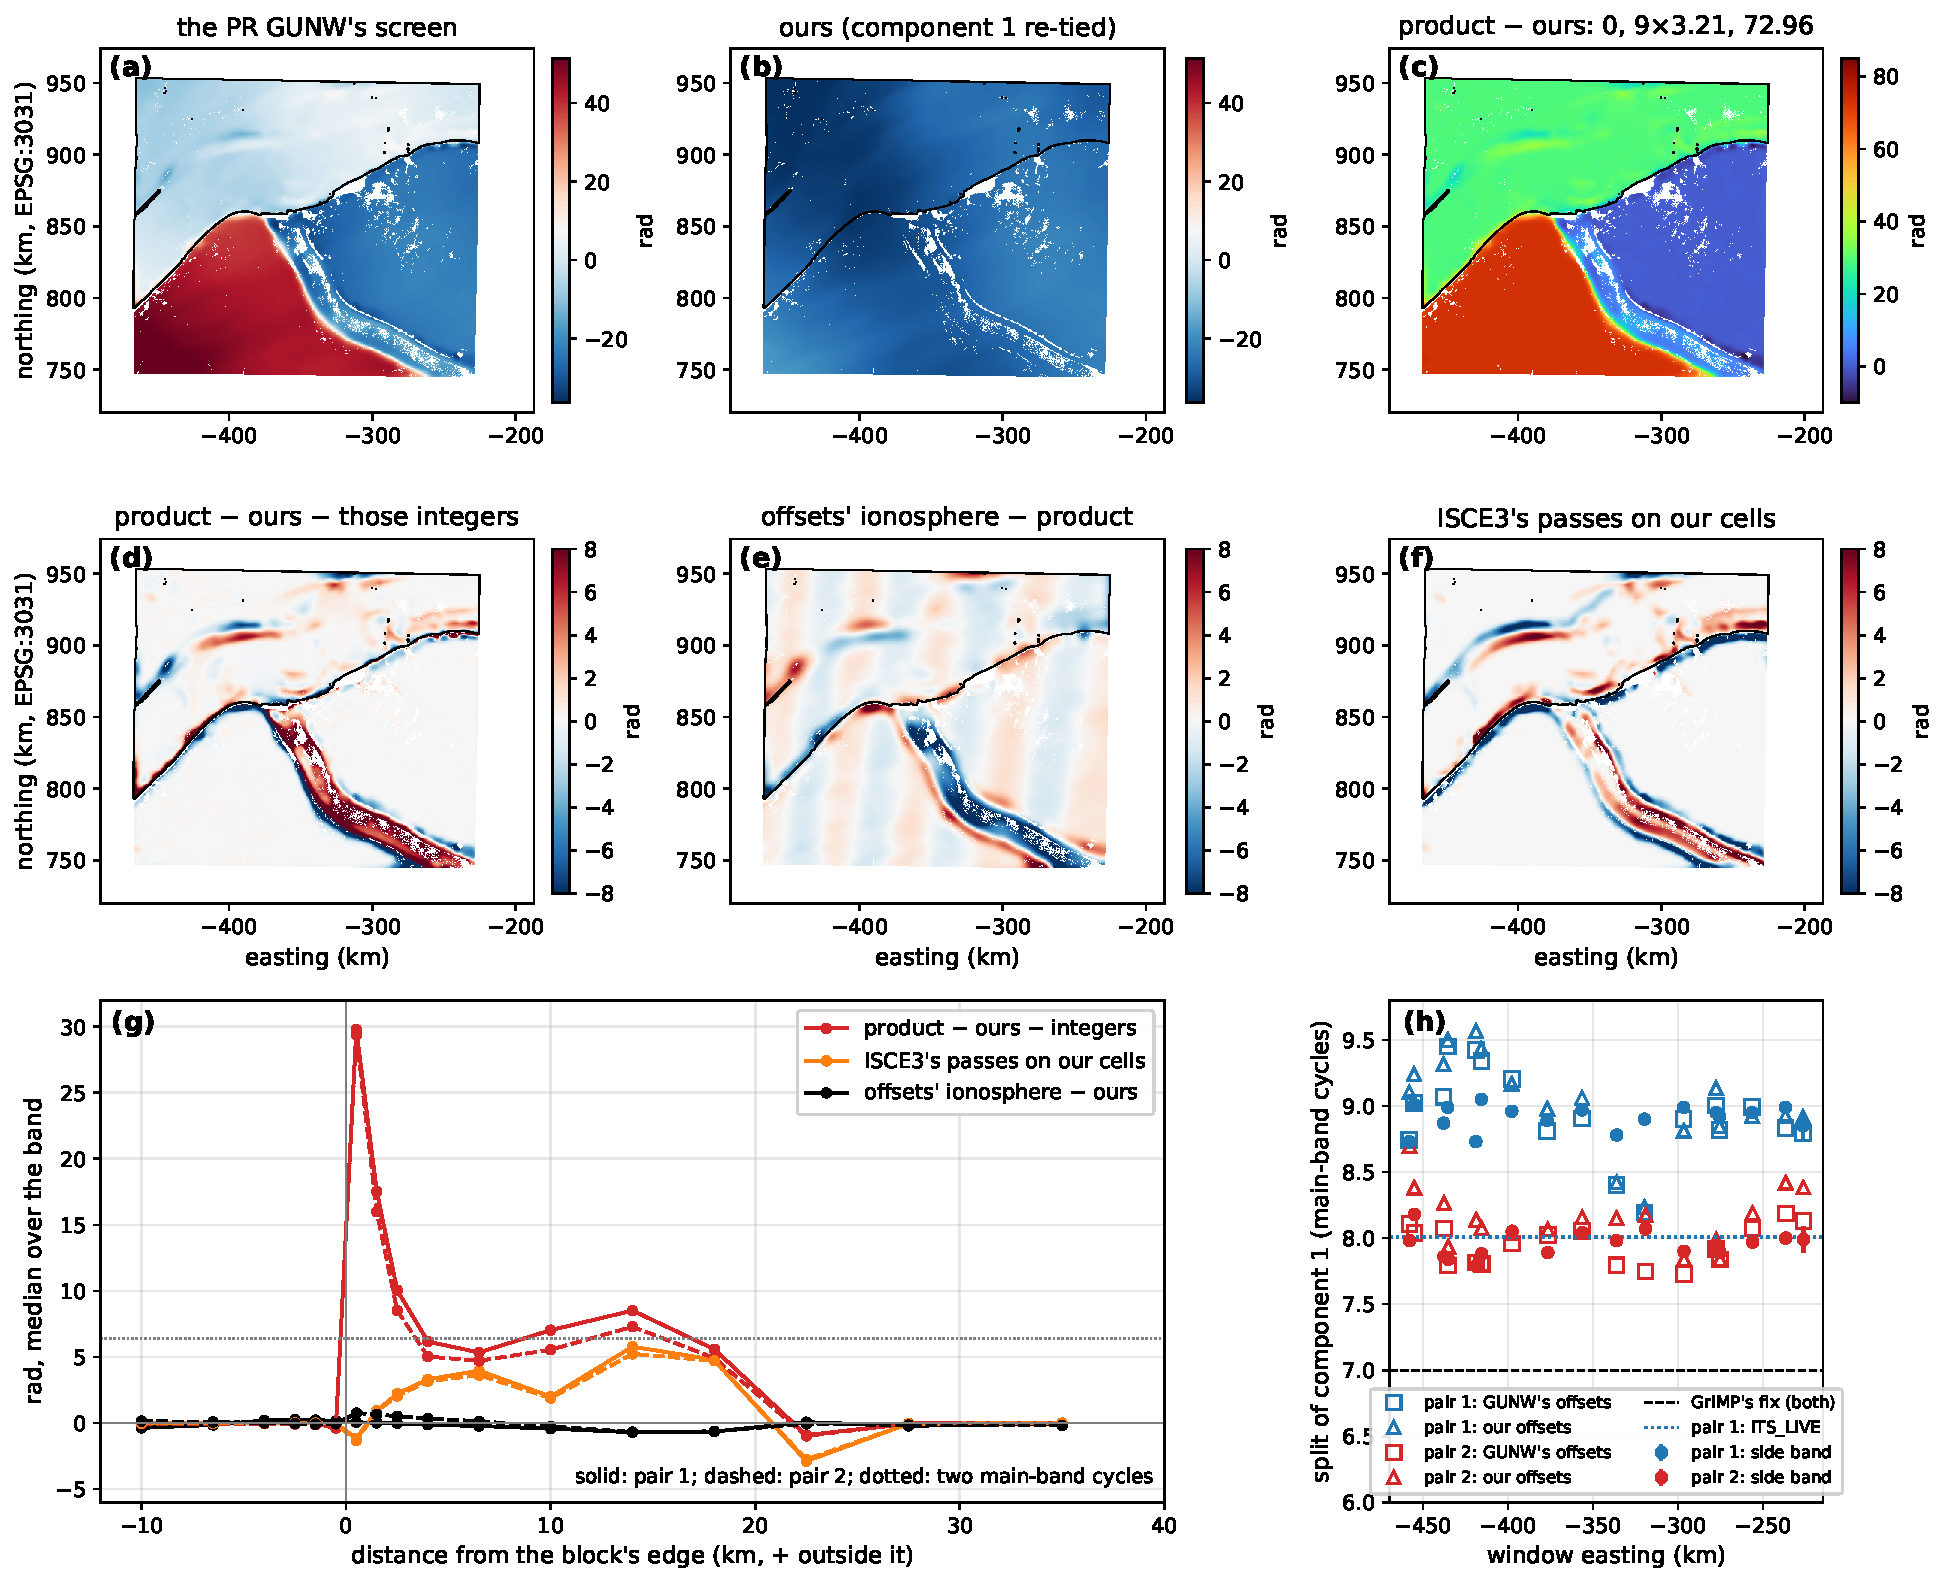
\includegraphics[width=\textwidth]{figures/fig_antarctica}
\caption{The Antarctic pair 19--31 August; pair 2 is alike (Table~\ref{tab:antarctica}).
(a) The PR GUNW's ionospheric screen. Black is the boundary between its connected components.
(b) Ours, with component 1 re-tied by the side band.
(c) Their difference takes three levels: 0; 9 main-band cycles (28.9\,rad) on component 1; and one cycle of the double
difference (73.0\,rad) over the block.
(d) What is left after those integers: the block's smeared edge, and the tributary's trunk.
(e) The offsets' ionosphere minus the product's screen, its integers repaired. The stripes are the offsets' own.
(f) What ISCE3's two correction passes add on our cells.
(g) Across the block's edge, median in bands parallel to it: the product's leftover, the passes on our cells, and the
offsets' ionosphere minus ours.
(h) The split of component 1 in the side band's 17 windows, by the side band and by the range offsets (the GUNW's and
our own), beside GrIMP's fix and ITS\_LIVE's reading.}
\label{fig:antarctica}
\end{figure}

\subsection{The product's screen is ours plus integers}
Product minus ours takes three levels (Fig.~\ref{fig:antarctica}c, Table~\ref{tab:antarctica}). Its baseline is the
densest $\pm5$\,rad window on component 2, because the block pulls that component's median.
\begin{itemize}
  \item On component 1 it is $+28.93$\,rad in pair 1 and $+25.69$\,rad in pair 2: 9.013 and 8.004 main-band cycles of
        3.21\,rad (robust sd 0.25 and 0.26). The product carries the main band's split between its components into its screen,
        as Table~\ref{tab:integers} says it must. Our tied screen does not step across the boundary: $-0.4$\,rad,
        2--8\,km either side, against the product's $+25.5$ and $+23.0$.
  \item Over a block of 11\,980 and 11\,304\,km$^2$ in component 2, between the component boundary and a tributary's
        western shear margin, it is $+73.00$ and $+72.92$\,rad in the block's core (robust sd 0.04): 1.0006 and 0.9995
        cycles of the double difference. This is the block that \citet{joughin2026nisarerrors} describe.
  \item Everywhere else it is 0.00\,rad (robust sd 0.07).
\end{itemize}
The block is the second mechanism of Section~\ref{sec:theory}. Decorrelated margins cut it off on both sides. The
non-dispersive phase steps across them by 167 and 120\,rad (3--6\,km either side, pair 1; pair 2 within 2\%), which puts
1.17 and 0.84 cycles into $\Delta$: more than $\pi$ across each gap. The product's unwrapping of $\Delta$ left the block
a cycle off both its neighbours. On our cells SNAPHU fails the same way, with the cycle on a different side: it puts
component 1 one cycle of $\Delta$ off, across the boundary where the step puts 1.06 cycles into $\Delta$. Ours unwraps
nothing that carries the flow.

\subsection{What is left after the integers}
After the integers, the screens still differ by more than 3\,rad over 5\,400 and 5\,078\,km$^2$
(Fig.~\ref{fig:antarctica}d). Two things make it (Fig.~\ref{fig:antarctica}g).
\begin{itemize}
  \item Within 3\,km outside the block's edge, the product is 17.7 and 16.4\,rad above ours (median). This is the
        product's filter smearing the block's 73\,rad step over a few kilometres, which no integer can repair.
  \item From 5 to 20\,km outside the block, over the tributary's trunk (1\,794 and 1\,820\,km$^2$), there is a plateau of
        6.50 and 5.44\,rad: 2.03 and 1.70 main-band cycles. The filter cannot smear that far.
\end{itemize}
The plateau is the first mechanism. We ran ISCE3's two correction passes (Section~\ref{sec:corrections}) on our cells,
with the main band tied. They move main-band cycles at 21\% of the cells, and over the plateau they raise the screen by
3.60 and 3.52\,rad (90th percentile 7.9). That is the product's place and sign, at about 60\% of its size
(Fig.~\ref{fig:antarctica}f).

Elsewhere the passes on our cells do more than the product shows: they are 18\,rad low where the product is 3\,rad low.
The passes ran on the product's own grid, which our cells do not reproduce, as on the Venezuela tracks
(Section~\ref{sec:nisar}). More than 5\,km from either integer step, the product's screen regresses on the 15\,km
high-pass of the non-dispersive phase at $-0.066$ ($r = -0.65$ and $-0.67$) in both pairs, and ours at $+0.002$ and
$+0.001$. That is the sign-flipped copy of Section~\ref{sec:intro}, here of the ice flow.

\subsection{Which screen is right over the fast ice}
The range offsets can tell. Phase advance and group delay have opposite signs, so $\phiA - k\rho_\mathrm{off}$ cancels
the flow and leaves twice the ionosphere, where $k = 4\pi\fA/c$ and $\rho_\mathrm{off}$ is the slant-range offset.
GrIMP's screen rests on the same physics \citep{joughin2026nisarerrors}. We use two sets of offsets. The GUNW's are
ISCE3's dense offsets (128-pixel windows every 75 pixels), culled, refilled and filtered for its rubbersheet. Our own come
from the same correlator ported to \texttt{nisar\_tools.roff} (64-pixel windows every 150 pixels), with only gross
outliers removed: those at the edge of the search, or more than 1\,m from the median of their $5\times5$
neighbourhood.

Smoothed over 3\,km, the offsets' ionosphere is calibrated on our screen where the two screens agree, as a slope plus a
plane. The slope is 2.01 and 1.83 with the GUNW's offsets, and 2.04 and 1.86 with ours, against 2 in theory. Where the
product departs, both sets follow our screen.
\begin{itemize}
  \item Where the product is more than 3\,rad above ours, the GUNW's offsets are $-0.28$ and $-0.32$\,rad from ours and
        $-5.60$ and $-4.91$\,rad from the product. Ours are $+0.11$ and $-0.20$ from ours and $-4.95$ and $-4.55$ from the
        product.
  \item Where the product is more than 3\,rad below ours, the GUNW's are $+0.34$ and $+0.27$ from ours and $+3.47$ and
        $+3.01$ from the product. Ours are $+0.26$ and $0.00$ from ours and $+3.31$ and $+2.73$ from the product.
\end{itemize}
(Table~\ref{tab:antarctica}; Fig.~\ref{fig:antarctica}e, g.) The product's departure does not scale with the unwrapped
phase ($R^2$ 0.03--0.04), so it is not a wrong frequency ratio.

\subsection{The components' split, three ways}
The side band ties component 1 at 8.95 cycles in pair 1 and 7.97 in pair 2. Each is the median of 17 windows along the
boundary, with a spread of 0.09. The range offsets, read the same way (a plane and a step in 30\,km windows at the same
17 places, using pixels 3--15\,km from the other component), give 8.90 and 7.96 with the GUNW's offsets, window by
window (Fig.~\ref{fig:antarctica}h). Our own offsets give 9.06 and 8.15 (spread 0.34 and 0.21).

Velocity maps read lower. ITS\_LIVE's version-2 mosaic \citep{gardner2018its,itslive2024v2}, on slow ice within 20\,km of
the boundary, reads 8.01 in pair 1. GrIMP's map reads the phase's step across the boundary as 7.5 cycles
\citep{joughin2026nisarerrors}. Component 2's side of the boundary is fast ice, so the nearest slow ice is across the
trunk, and a velocity map's error there enters the tie whole. The split is therefore 9 and 8 cycles, and GrIMP's $-7$
leaves component 1 two and one cycles off in the unwrapped phase. A residual metric that removes each component's
median cannot show that.

This boundary is also the control that Section~\ref{sec:sbtie} lacked. The non-dispersive phase steps across it by
74--188\,rad (median 162\,rad, 3.1\,m of LOS), as much as across the Panama ruptures. There the side band agrees with a
tie that shares none of its assumptions, so a bias of the side band that grew with the step would show up here as a
cycle. This is one look direction, descending.

\subsection{How good each correction is}
Three measures score the corrected phase, $\phiA$ minus a screen (Table~\ref{tab:antarctica}). The first two need no
velocity map.

\paragraph{Against the offsets' ionosphere.} With the phase tied, $(\phiA - k\rho_\mathrm{off})/2$ is an ionosphere
estimate independent of both screens, and here nothing is calibrated on either. It and each screen are smoothed over
6\,km, and a median and a plane are removed per screen. Our screen then departs from it by 0.63 and 0.68\,rad rms
(1.2--1.3\,cm of LOS). The product's screen misses it by 18.9\,rad as delivered, mostly through its integers. Once they
are repaired it misses by 1.29 and 1.21\,rad, twice ours, from the trunk's plateau and the smeared block edges.

\paragraph{Pair consistency.} Both pairs span 12 days on one track, so for steady flow their corrected phases should
match. Pair 1 minus pair 2, with a median and a plane removed, leaves what the corrections missed, noise, and any change
in the flow; 6.6 million pixels are coherent in both. Uncorrected it is 3.94\,rad (robust 4.13), the ionosphere that
changed between the pairs. Both screens remove most of it: the product's leaves 1.30 (0.99), ours 1.02 (0.81).

This measure cannot see errors that repeat in both pairs, and the product's do: the same block, splits of 9 and 8
cycles, the same plateau. That is why the product scores nearly as well as ours here. (Its repaired version scores 2.70,
because the repair of the smeared block edges differs between the pairs.) Faint stripes remain under both screens. The
carrier error of \citet{joughin2026nisarerrors}, which no screen removes, is a candidate; we have not tested it.

\paragraph{Against a velocity synthetic.} We also computed \citet{joughin2026nisarerrors}'s own metric: the phase minus a synthetic interferogram, with each
component's median and a plane removed. The synthetic comes from ITS\_LIVE's 120\,m static mosaic, projected on the
GUNW's line of sight over 12 days, with surface-parallel vertical flow. Pixels need coherence above 0.3 and grounded ice.

The multi-year mosaic misses the fast trunks: the product's corrected phase regresses on it at 0.40 above 200\,m/yr.
So only slow ice ($<$50\,m/yr), where the slope is 0.998 and 0.994, is meaningful.
\begin{itemize}
  \item Our screen leaves 1.84\,rad there in both pairs (robust 1.22 and 1.21).
  \item The uncorrected phase leaves 3.50 and 2.09 (3.15 and 1.69).
  \item The product's screen leaves 15.2 and 15.1 (14.2 and 14.1).
  \item Repairing the product's integers brings it to 4.0 (1.4); the smear and the trunk's cycles remain.
\end{itemize}
These numbers cannot be compared with those of \citet{joughin2026nisarerrors}, which use GrIMP's velocity map over all
ice with coherence above 0.3.

\subsection{What the Antarctic pairs show}
Each way the integers can go wrong in Section~\ref{sec:theory} appears in these products, in whole cycles.
\begin{itemize}
  \item The main band's split between its components is carried at 3.21\,rad per cycle: 9 and 8 cycles.
  \item One cycle of the double difference was unwrapped across decorrelated margins: 73\,rad over 12\,000\,km$^2$.
  \item The correction passes moved about two main-band cycles over a fast trunk.
\end{itemize}
None of this needs an earthquake: a glacier's shear margins are enough. The reordered estimate avoids the second and
third by construction, and the side band, checked here by the range offsets, repairs the first. Wherever the two can be
compared, our screen then agrees with the offsets' ionosphere to a few tenths of a radian.

\section{Discussion}
\label{sec:discussion}

\subsection{Where the deformation enters}
Three mechanisms put deformation into a split-spectrum screen, and the experiments separate them.
\begin{enumerate}
  \item \emph{Cycle corrections.} Rounding an unwrapped field against its own low-pass, or against the filtered
        first-pass estimates, reads the deformation's curvature as unwrapping errors. Each false cycle of the main
        band is 3.21\,rad of screen, and the false cycles follow the deformation. The result is a fixed fraction of
        it, $-0.045$ to $-0.048$ on our synthetics and $-0.06$ without an exclusion, whatever the slip or the
        geometry. This is the sign-flipped copy the GUNW screens show. It needs no unwrapping error at all: the passes
        create the errors they correct. They also act at data edges, where their one-sided low-pass lags any steep
        gradient (Appendix~\ref{app:isce3}).
  \item \emph{Unwrapping a field that carries deformation across a rupture that splits the scene.} The side band
        carries all of the step and the double difference 4.4\% of it. Once that share exceeds about $\pi$, the
        cross-fault integer is a guess. The guess is wrong by one cycle of $\Delta$ (73\,rad, 1.4\,m of LOS) on D141,
        whose 3.8\,m step puts 1.38 cycles into $\Delta$, and on our synthetics from 4--6\,m of slip on. Where the
        unwrapper can go around the rupture's ends, this does not happen.
  \item \emph{Band co-location.} A side band sampled $\delta$ down range adds $12.1\,\delta$ times the deformation's
        range gradient. For strike-slip ruptures that a polar-orbiting SAR sees, the gradient mostly runs along
        azimuth, and ISCE3's 9\,m offset is worth well under a millimetre beyond 2\,km. Close to the trace, or for a
        rupture whose gradient points down range, it is centimetres.
\end{enumerate}
The reordered estimator removes the first two by construction, because its unwrapped field carries no deformation,
and the third by summing both bands over identical cells. The Antarctic pairs (Section~\ref{sec:antarctica}) show the
first two, and the products' main-band integers below, without an earthquake. Across a glacier's shear margins their
screen is ours plus:
\begin{itemize}
  \item one cycle of $\Delta$ over a 12\,000\,km$^2$ block;
  \item the main band's split between its components;
  \item about two main-band cycles that the passes moved over a fast trunk.
\end{itemize} What its screen still contains near a rupture is the
filter's (next subsection), and that is the same with and without the rupture.

The products add a fourth, which no split-spectrum form avoids: the main band's own integers. On D141 the PR GUNW's
main band is 25 cycles off on the cut-off block and 3--9 cycles off north of the trace. Those integers alone make our
estimate leak $-0.061$. On the Venezuela tracks the products' main band agrees with ours, and the recipe on our cells
accounts for 25--52\% of the products' leak beyond ours. Matching the products' side-band footprint changes that by
at most 0.004. The rest is in steps our matched cells do not reproduce.

\subsection{What the reordering does not remove}
\label{sec:tie}
\paragraph{The main band's integers.} The reordered estimate needs $\phiA$ unwrapped correctly, and so does the
deformation it serves. A cycle of $\phiA$ moves the raw estimate by $2\pi c_0 = 3.21$\,rad, about 62\,mm of LOS,
exactly as in the reformulated form. On the D141 pair, where SNAPHU's default and ``defo'' costs chose different
integers in a few patches, the raw estimate moved by exactly 3.21\,rad per cycle. A block that the cut isolates needs
its own integer. The range offsets give one: $m = (4\pi/\lambda)\,\rho_\mathrm{off} - \phiA$ holds no deformation, only
the block's cycles plus twice the ionosphere, because offsets see the ionosphere as a delay and phase as an advance.
Combining $m$ with the screen does not help: $m + 2\hat\phi_{io}$ moves only 0.022 cycles per cycle of the tie
\citep[Sec.~III-D makes the same point about phase--group-delay differences]{gomba2016toward}, and the bands' absolute
(``delta-$k$'') phase \citep{bovenga2013mca} is as much ionosphere as integer. The screen's own continuity across the
gap does settle it, to about a tenth of a cycle, and finds the pipelines' offset ties a cycle short on three of the
four Panama pairs (Section~\ref{sec:sbtie}). The offsets were not wrong; the pipelines' reading of them was. They
compared separate planes, fitted 6--12\,km from the trace on each side, at the trace. Read with the side band's
estimator, the same offsets agree with it to a third of a cycle. Across an Antarctic shear margin the non-dispersive phase steps by 74--188\,rad. There
the side band and the range offsets agree to 0.05 cycles, and both find the operational velocity-map fix one or two
cycles short (Section~\ref{sec:antarctica}). Far from the trace a wrong tie shifts the block's corrected LOS by a constant
59\,mm, which a per-block offset in the inversion absorbs. Near the trace the filter fills the excluded zone from both
sides and mixes them, leaving a fake step of 5--6\,cm per cycle that decays over $\sim$8\,km
(Fig.~\ref{fig:tie}d). Filtering each block separately would remove the mixing at the cost of the north side's sparse
near-trace cells.

\paragraph{The cells, the fill and the filter.} Near a rupture three parts of the estimator add error that has nothing
to do with the slip (Section~\ref{sec:nearfield}). The cells sum steep fringes differently in the two bands; the fill
of the excluded zone is a plane wider than the zone; and ISCE3's weighted mean lags the ionosphere's gradient where
the damage zone lowers the weights. On the synthetics each can be removed, by taking the main band out of every pixel,
by a fill matched to the gap and by a weighted local plane as the final step, and together they bring the error within
2\,km of the trace from 16 to 2\,mm. On real data they matter less. Real ionosphere is smoother at 2--10\,km than our
synthetics, and the fills differ by about a millimetre in a 2\,km fault zone. On D141 the plane moves the screen by at
most 3\,mm.

\paragraph{The main band's local integers.} What does matter on D141 is the main band near the trace. Its cut and uncut
unwrappings disagree on 18--78\% of the cells within 6\,km north of the trace, at 3.21\,rad of raw estimate per cycle.
Every recipe that follows the near-trace cells more closely takes those disagreements into the screen: up to 16\,mm
for the narrow fills, against 2.4\,mm or less for the production screen, whose 10\,km fill averages them away. The
production recipe's wide fill and its 2\,km exclusion are therefore the robust choice until the integers near a trace
can be checked. The side band could check them patch by patch, as it ties a cut-off block.

\paragraph{Strong ionosphere.} $r = k\,\phi_{io}$ wraps once $\phi_{io}$ changes by $2\pi/|k| = 73$\,rad. Unwrapping it
fails only if it changes by $\pi$ between neighbouring cells, about 36\,rad of ionosphere per 240\,m cell, or six cycles
of $\phiA$ per cell. The main band fails long before that. On the steepest of our screens (D126), $r$ spans about
10\,rad over the scene.

\paragraph{What it does not address.} Azimuth streaks from ionospheric scintillation, the registration errors that
ionospheric azimuth shifts cause \citep{wegmuller2024palsar3}, and the higher-order terms some sporadic-E cases need
\citep{furuya2017midlatitude} are beyond this paper. The reordering changes only what is unwrapped. It is compatible
with any filter, with the Bayesian combination of \citet{gomba2017bayesian}, and with time-series estimation
\citep{fattahi2017insar,piromthong2026ionospheric}.

\subsection{A one-line change for the operational products}
ISCE3 forms the double difference as the main-band interferogram times the conjugate of the side band's, and unwraps
it. Multiplying that product by $\exp\!\left(i\,\frac{\Delta f}{\fA}\,\phiA\right)$, using the main band's unwrapped
phase on the side band's grid, before unwrapping, and dividing it out afterwards, turns \eqref{eq:reform} into
\eqref{eq:ours} with no other change. With that, the correction passes have nothing left to correct near a rupture
and can be switched off there. The main band's own unwrapping across the rupture still matters, at 3.21\,rad of
raw estimate per cycle. The PR GUNW's unwrapped phase is 32 cycles off across the D141 rupture, because SNAPHU went
around its end, so a product that adopted the reordering would still need the rupture cut, or another way of
fixing that integer.

\section{Conclusions}
\label{sec:conclusions}
\begin{enumerate}
  \item The split-spectrum screens of NISAR's PR GUNWs copy the coseismic deformation near the 2026 Panama and
        Venezuela ruptures with the opposite sign. Within 10\,km of the trace, the screen's high-pass regresses on
        the data's at $-0.02$ to $-0.12$ ($r$ down to $-0.82$). On Panama's D141 pair the screen also steps 0.43\,m
        across the trace.
  \item On identical cells, with an identical filter and main-band unwrapping, two mechanisms account for most of it.
        \begin{itemize}
          \item The whole-cycle corrections read the deformation's curvature as unwrapping errors, and copy
                4.5--4.8\% of the high-passed deformation at any slip.
          \item Unwrapping a field that carries deformation (the side band, or the double difference) fails across a
                rupture that splits the scene: by one cycle of the double difference (1.4\,m of LOS) on D141.
        \end{itemize}
        On D141 the product's own main band, 25--32 cycles off across the rupture, carries most of its copy. On the
        Venezuela tracks, the corrections on matched cells reproduce 25--52\% of the products' leak beyond ours, and
        neither the main band nor the bands' footprint mismatch explains the rest.
  \item Removing the scaled, unwrapped main band from the wrapped side band before anything is unwrapped gives the
        same estimate as the reformulated split spectrum and the GUNW's, with nothing in the unwrapped field for an
        unwrapper or a correction to mistake. On every synthetic its error near the rupture stays at its zero-slip
        level. It needs the main band unwrapped correctly, as the deformation does, and a cut-off block's tie carries
        into the screen at 3.21\,rad per cycle.
  \item The same 3.21\,rad per cycle ties a block that a cut along the rupture isolates. The raw estimate's step across
        the gap reads the block's integer wherever the ionosphere is smooth over 10--20\,km: the median over 20\,km
        windows read no wrong integer on 565 fake boundaries in eight scenes, and 0.02 across a Venezuela rupture whose
        integer is known. On three Panama pairs it finds the pipelines' range-offset ties a cycle short. Read with the same
        estimator, the offsets agree with it: the pipelines' far-field planes were at fault, not the offsets. Ionospheric waves, and
        local cycle errors in a third of the cells beside the gap, bias it by a few tenths of a cycle; two estimators
        that fail differently, a polynomial and kriging, check each other.
  \item What remains near the fault on the synthetics, the same with and without the rupture, is the cells' handling of
        steep fringes, the fill's width and the lag of ISCE3's weighted mean across the damage zone. Taking the main
        band out of every pixel, matching the fill to the gap and making the filter's final step a weighted local
        plane bring it from 16 to 2\,mm within 2\,km of the trace. On real data these are millimetre corrections.
        Next to the D141 rupture the screen is limited by the main band's local integers, which the narrower recipes
        follow and the production screen's wide fill averages away.
  \item On two Antarctic pairs the operational screen is ours plus whole cycles:
        \begin{itemize}
          \item the main band's split between its components, 9 and 8 cycles;
          \item one cycle of the double difference over 12\,000\,km$^2$ beside a glacier's shear margins;
          \item about two main-band cycles from the correction passes over a fast trunk.
        \end{itemize}
        Where the screens differ beyond those integers, the range offsets side with ours. They also tie the components as
        the side band does across a 160\,rad step, where velocity maps read one to two cycles low.
  \item For the operational processor the change is one line: multiply the double difference by
        $\exp(i\,\Delta f\,\phiA/\fA)$ before unwrapping, and divide it out after. The rupture still needs a cut, and
        the side band then ties the blocks.
\end{enumerate}


\section*{Code and data availability}
The estimator is \texttt{nisar\_tools.split\_spectrum}, the side-band tie its \texttt{block\_cycles}, and the
near-trace options of Section~\ref{sec:nearfield} the \texttt{phase\_model} of its \texttt{gslc\_cells} and the
\texttt{fill\_m} ladder and \texttt{order} of its \texttt{ionosphere\_filter}; the
experiments of this paper, the synthetic generator and the
scripts that make every figure and table are in \texttt{docs/\allowbreak ionosphere\_paper/\allowbreak experiments/} of the
same repository.
The Antarctic pipeline of Section~\ref{sec:antarctica} (\texttt{ant\_pipeline.py}, \texttt{tie\_check.py},
\texttt{ant\_roff.py}) is beside its data, as the Panama and Venezuela pipelines are; \texttt{run\_antarctica.py} reads
it. The NISAR PR GSLC, RSLC and GUNW products are distributed by the Alaska Satellite Facility, and the ITS\_LIVE
velocity mosaics by the NSIDC DAAC.

\bibliographystyle{abbrvnat}
\bibliography{references}

\appendix
\section{Registration of the GSLC pairs}
\label{app:registration}
The PR GSLCs of the two dates are each geocoded with their own ionospheric (TEC) and solid-earth-tide geolocation
corrections. Those corrections differ between dates by about a resolution cell (2.5--3.2\,m on the Panama D141 pair),
so an interferogram formed directly from two GSLCs loses about half its coherence. We keep the first date's GSLC and
geocode the second date's RSLC onto its grids. That geocoding drops the second date's own corrections and adds a
registration field: the first date's correction shift plus the offsets measured between the two dates (our port of
ISCE3's ROFF correlator). The side band is geocoded with the same field in its own pixels; the TEC part of the shift
scales by $(\fA/\fB)^2$. Both bands of both dates then lie on common grids, and the cells of
Section~\ref{sec:estimator} are sums over identical pixels.

\section{ISCE3's correction passes, as ported}
\label{app:isce3}
With $\mathcal{G}$ a NaN-aware truncated Gaussian ($\sigma$ 2.0\,km by 2.6\,km, truncated at 1.75 and 1.49 $\sigma$:
ISCE3's 14 by 110 taps for $\sigma$ 4 by 37 side-band pixels), the first pass
(\texttt{unwrapping\_correction\_with\_filter}, one iteration) replaces every unwrapped field $u$ ($\phiA$ and
$\Delta$, or $\phiA$ and $\phiB$) by
\begin{equation}
  u \leftarrow u - 2\pi \left\lfloor \frac{u - \mathcal{G}u}{2\pi} \right\rceil .
\end{equation}
The second pass (\texttt{compute\_unwrapp\_error\_main\_diff\_ms\_band}) forms the first estimates
$\hat d = c_0\phiA + c_1\Delta$ and $\hat n = \phiA - \hat d$, filters both with the dispersive filter ($F$), and
corrects
\begin{equation}
  \phiA \leftarrow \phiA - 2\pi\left\lfloor\frac{\phiA - F\hat n - F\hat d}{2\pi}\right\rceil,\qquad
  \Delta \leftarrow \Delta - 2\pi\left\lfloor\frac{\Delta + \frac{\Delta f}{\fA}F\hat n - \frac{\Delta f}{\fB}F\hat d}
  {2\pi}\right\rceil ,
\end{equation}
before the final estimate and filter. The two-band version
(\texttt{compute\_unwrapp\_error\_main\_side\_band}) rounds the differential integer
$\lfloor[(1-\fB/\fA)F\hat n + (1-\fA/\fB)F\hat d + \phiB - \phiA]/2\pi\rceil$ and the common one from the sum, as in
\citet[eqs.~28--29]{gomba2016toward}. ISCE2's ALOS-2 processor instead rounds $\phiA-\phiB$ against a weighted
quadratic of itself \citep{liang2018insar}. These are the \texttt{diff\_isce3}, \texttt{side\_isce3} and
\texttt{side\_isce2} estimators of the experiments.

\section{The synthetic generator}
\label{app:synthetic}
The scene is 96 by 96\,km of 40\,m pixels. The truth is a vertical left-lateral rupture striking N105$^\circ$E,
built from Okada rectangles \citep{okada1985surface}: 10 segments along strike by two in depth (0--10 and 10--15\,km;
the lower layer carries 0.6 of the slip), with slip tapered along strike as $\sqrt{\sin}$. It is 50\,km long and ends
inside the scene (``finite''), or 160\,km long and runs through it (``through''). The LOS is a left-looking
descending pass at 37$^\circ$ incidence, D141's geometry. The ionosphere, at $\fA$, is a 0.6\,rad/km gradient plus a
Gaussian-correlated field (rms 4\,rad, correlation length 15\,km), about 80\,rad across the scene.

Each band's coherence is a far-field value (0.6, or 0.35) times a damage zone, $q + (1-q)(1-e^{-(d/w)^2})$ with
$q\gamma_0 = 0.12$ and $w=2$\,km north of the trace and $q\gamma_0=0.25$, $w=0.8$\,km south (close to D141's
measured coherence), times the fringe-rate loss $|\mathrm{sinc}|$ of the band's own phase gradient \citep{zebker1992decorrelation}. That loss is
taken over the band's resolution cell (6.2\,m of ground range for the main band, 50\,m for the side band, 5.3\,m
along track) and over the 40\,m pixel.

Each pixel's interferometric sum of $L$ looks (48 for the main band, 6 for the side band) is drawn from the complex
Wishart distribution with that coherence and phase, by the Bartlett decomposition \citep{lee1994intensity}. With
$g_1\sim\Gamma(L)$, $g_2\sim\Gamma(L-1)$ and $a\sim\mathcal{CN}(0,1)$,
\begin{equation}
  \begin{aligned}
  W_{12} &= g_1\gamma e^{i\phi} + \sqrt{g_1}\,\bar a\,\sqrt{1-\gamma^2}, \qquad W_{11} = g_1,\\
  W_{22} &= \gamma^2 g_1 + 2\,\mathrm{Re}\!\left(\gamma e^{-i\phi}\sqrt{g_1}\,\bar a\sqrt{1-\gamma^2}\right)
  + (1-\gamma^2)(|a|^2+g_2).
  \end{aligned}
\end{equation}
The pixels are summed over 240\,m cells exactly as GSLC pixels are, which gives 1728 and 216 looks per cell
(\texttt{split\_spectrum}'s own estimate for NISAR's 40\,+\,5\,MHz mode: 1753 and 217). The main band's unwrapping is
the oracle: the cell mean of the true phase, with the noisy cell phase re-wrapped onto it. All estimators therefore
see the same, correct $\phiA$, and differ only in how they use the side band.


\end{document}
